%%% The main file. It contains definitions of basic parameters and includes all other parts.

% Meta-data of your thesis (please edit)
\input metadata.tex

% Generate metadata in XMP format for use by the pdfx package
\input xmp.tex

%% Settings for single-side (simplex) printing
% Margins: left 40mm, right 25mm, top and bottom 25mm
% (but beware, LaTeX adds 1in implicitly)
\documentclass[12pt,a4paper]{report}
\setlength\textwidth{145mm}
\setlength\textheight{247mm}
\setlength\oddsidemargin{15mm}
\setlength\evensidemargin{15mm}
\setlength\topmargin{0mm}
\setlength\headsep{0mm}
\setlength\headheight{0mm}
% \openright makes the following text appear on a right-hand page
\let\openright=\clearpage

%% Settings for two-sided (duplex) printing
% \documentclass[12pt,a4paper,twoside,openright]{report}
% \setlength\textwidth{145mm}
% \setlength\textheight{247mm}
% \setlength\oddsidemargin{14.2mm}
% \setlength\evensidemargin{0mm}
% \setlength\topmargin{0mm}
% \setlength\headsep{0mm}
% \setlength\headheight{0mm}
% \let\openright=\cleardoublepage

%% If the thesis has no printed version, symmetric margins look better
% \documentclass[12pt,a4paper]{report}
% \setlength\textwidth{145mm}
% \setlength\textheight{247mm}
% \setlength\oddsidemargin{10mm}
% \setlength\evensidemargin{10mm}
% \setlength\topmargin{0mm}
% \setlength\headsep{0mm}
% \setlength\headheight{0mm}
% \let\openright=\clearpage

%% Generate PDF/A-2u
\usepackage[a-2u]{pdfx}

%% Prefer Latin Modern fonts
\usepackage{lmodern}
% If we are not using LuaTeX, we need to set up character encoding:
\usepackage{iftex}
\ifpdftex
\usepackage[utf8]{inputenc}
\usepackage[T1]{fontenc}
\usepackage{textcomp}
\fi

%% Further useful packages (included in most LaTeX distributions)
\usepackage{amsmath}        % extensions for typesetting of math
\usepackage{amsfonts}       % math fonts
\usepackage{amsthm}         % theorems, definitions, etc.
\usepackage{bm}             % boldface symbols (\bm)
\usepackage{booktabs}       % improved horizontal lines in tables
\usepackage{caption}        % custom captions of floating objects
\usepackage{dcolumn}        % improved alignment of table columns
\usepackage{floatrow}       % custom float environments
\usepackage{graphicx}       % embedding of pictures
\usepackage{indentfirst}    % indent the first paragraph of a chapter
\usepackage[nopatch=item]{microtype}   % micro-typographic refinement
\usepackage{paralist}       % improved enumerate and itemize
\usepackage[nottoc]{tocbibind} % makes sure that bibliography and the lists
			    % of figures/tables are included in the table
			    % of contents
\usepackage{xcolor}         % typesetting in color

% The hyperref package for clickable links in PDF and also for storing
% metadata to PDF (including the table of contents).
% Most settings are pre-set by the pdfx package.
\hypersetup{unicode}
\hypersetup{breaklinks=true}

% Packages for computer science theses
\usepackage{algpseudocode}  % part of algorithmicx package
\usepackage{algorithm}
\usepackage{fancyvrb}       % improved verbatim environment
\usepackage{listings}       % pretty-printer of source code

% You might want to use cleveref for references
% \usepackage{cleveref}

% UNCOMMENT THIS IF THERE IS AN ERROR IN THE BIBLIOGRAPHY
% \DeclareUnicodeCharacter{0301}{*************************************}

% Set up formatting of bibliography (references to literature)
% Details can be adjusted in macros.tex.
%
% BEWARE: Different fields of research and different university departments
% have their own customs regarding bibliography. Consult the bibliography
% format with your supervisor.
%
% The basic format according to the ISO 690 standard with numbered references
%\usepackage[natbib,style=iso-numeric,sorting=none]{biblatex}
% ISO 690 with alphanumeric references (abbreviations of authors' names)
%\usepackage[natbib,style=iso-alphabetic]{biblatex}
% ISO 690 with references Author (year)
%\usepackage[natbib,style=iso-authoryear]{biblatex}

% Using standard numeric style instead due to compatibility issues with iso style
\usepackage[natbib,style=numeric,sorting=none]{biblatex}
% TODO: look at the citation styles once more...

%
% Some fields of research prefer a simple format with numbered references
% (sorting=none tells that bibliography should be listed in citation order)
%\usepackage[natbib,style=numeric,sorting=none]{biblatex}
% Numbered references, but [1,2,3,4,5] is compressed to [1-5]
%\usepackage[natbib,style=numeric-comp,sorting=none]{biblatex}
% A simple format with alphanumeric references:
%\usepackage[natbib,style=alphabetic]{biblatex}

% Load the file with bibliography entries
\addbibresource{bibliography.bib}

% Our definitions of macros (see description inside)
\input macros.tex

%%% Title page and various mandatory informational pages
\begin{document}
%%% Title page of the thesis and other mandatory pages

%%% Inscriptions at the opening page of the hard cover

% We usually do not typeset the hard cover, but if you want to do it, change \iffalse to \iftrue
\iffalse

\pagestyle{empty}
\hypersetup{pageanchor=false}
\begin{center}

\large
Charles University

\medskip

Faculty of Mathematics and Physics

\vfill

{\huge\bf\ThesisTypeTitle}

\vfill

{\huge\bf\ThesisTitle\par}

\vfill
\vfill

\hbox to \hsize{\YearSubmitted\hfil \ThesisAuthor}

\end{center}

\newpage\openright
\setcounter{page}{1}

\fi

%%% Title page of the thesis

\pagestyle{empty}
\hypersetup{pageanchor=false}
\begin{center}

\centerline{\mbox{
\includegraphics[width=166mm]{img/logo-en.pdf}}}

\vspace{-8mm}
\vfill

{\bf\Large\ThesisTypeTitle}

\vfill

{\LARGE\ThesisAuthor}

\vspace{15mm}

{\LARGE\bfseries\ThesisTitle\par}

\vfill

\Department

\vfill

{
\centerline{\vbox{\halign{\hbox to 0.45\hsize{\hfil #}&\hskip 0.5em\parbox[t]{0.45\hsize}{\raggedright #}\cr
Supervisor of the \ThesisTypeName{} thesis:&\Supervisor \cr
\ifx\ThesisType\TypeRig\else
\noalign{\vspace{2mm}}
Study programme:&\StudyProgramme \cr
\fi
}}}}

\vfill

Prague \YearSubmitted

\end{center}

\newpage

%%% A page with a solemn declaration to the thesis

\openright
\hypersetup{pageanchor=true}
\vglue 0pt plus 1fill

\noindent
I declare that I carried out this \ThesisTypeName{} thesis on my own, and only with the cited
sources, literature and other professional sources.
I understand that my work relates to the rights and obligations under the Act No.~121/2000 Sb.,
the Copyright Act, as amended, in particular the fact that the Charles
University has the right to conclude a license agreement on the use of this
work as a school work pursuant to Section 60 subsection 1 of the Copyright~Act.

\vspace{10mm}

\hbox{\hbox to 0.5\hsize{%
In \hbox to 6em{\dotfill} date \hbox to 6em{\dotfill}
\hss}\hbox to 0.5\hsize{\dotfill\quad}}
\smallskip
\hbox{\hbox to 0.5\hsize{}\hbox to 0.5\hsize{\hfil Author's signature\hfil}}

\vspace{20mm}
\newpage

%%% Dedication

\openright

\noindent
\Dedication

\newpage

%%% Mandatory information page of the thesis

\openright
{\InfoPageFont

\vtop to 0.5\vsize{
\setlength\parindent{0mm}
\setlength\parskip{5mm}

Title:
\ThesisTitle

Author:
\ThesisAuthor

\DeptType:
\Department

Supervisor:
\Supervisor, \SupervisorsDepartment

Abstract:
\Abstract

Keywords:
{\def\sep{\unskip, }\ThesisKeywords}

\vfil
}

% In Czech study programmes, it is mandatory to include Czech meta-data:

\ifx\StudyLanguage\LangCS

\vtop to 0.49\vsize{
\setlength\parindent{0mm}
\setlength\parskip{5mm}

Název práce:
\ThesisTitleCS

Autor:
\ThesisAuthor

\DeptTypeCS:
\DepartmentCS

Vedoucí práce:
\Supervisor, \SupervisorsDepartmentCS

Abstrakt:
\AbstractCS

Klíčová slova:
{\def\sep{\unskip, }\ThesisKeywordsCS}

\vfil
}

\fi

}

\newpage

%%% Further pages will be numbered
\pagestyle{plain}


%%% A page with automatically generated table of contents of the thesis

\tableofcontents

%%% Each chapter is kept in a separate file
\chapter*{Introduction}
\addcontentsline{toc}{chapter}{Introduction}

Proteins are essential to a wide range of biological processes. Proteins consist of amino acids, which are the building blocks of these macromolecules. The amino acids form a chain that determines the protein's structure and function. Certain amino acids, referred to as binding, are more likely to interact with other molecules called ligands. This is a fundamental property to drug discovery and research \cite{trainor2007importance}, \cite{ballante2021protein}, \cite{mannhold2006protein}.

Detection of such residues, which are individual amino acids within the protein structure, is a challenging task, and various computational methods have been developed to predict potential binding residues, which are further grouped into distinct binding regions (also referred to as binding sites) based on the location of the residues \cite{krivak2018p2rank}, \cite{le2009fpocket}, \cite{aggarwal2021deeppocket}, \cite{smith2024graph}. Certain binding residues may experience structural changes due to the dynamic nature of these regions, becoming cryptic binding residues (CBRs) that pose greater identification challenges. While current methods may detect cryptic binding sites (CBSs), their models are generally trained to identify any binding residues, rather than being specifically focused on CBSs.

A dataset and methodology for detecting CBRs was previously developed at the Faculty of Mathematics and Physics, Charles University, known as CryptoBench \cite{vskrhak2025cryptobench}. This thesis has two primary objectives. 

The first goal is to extend this approach by clustering individually predicted CBRs from the CryptoBench model into structurally contiguous regions, referred to as CBSs. This methodology may also be applicable to other prediction methods.

The second objective is to develop a user-friendly client-server web application, CryptoShow, which would enable users to submit protein structures and obtain CBR predictions. These predictions would be clustered into distinct binding sites and visualized for the user, including animations that illustrate potential conformational changes between the protein's initial state and analogous structures identified using the AHoJ tool \cite{feidakis2022ahoj}.

This thesis is structured in four chapters, and it is organized as follows:

Chapter 1 provides an overview of the field of bioinformatics, introducing key terminology, concepts, and relevant tools that underpin the subsequent work.

Chapter 2 details the methodological framework, beginning with the prediction of cryptic binding residues using the CryptoBench model. This is followed by a description of the clustering approach for grouping CBRs into cryptic binding sites, and concludes with an explanation of the animation pipeline for visualizing conformational transitions between protein structures.

Chapter 3 presents the design and implementation of the CryptoShow web application. This includes a discussion of the technology stack, architectural and design choices, and an in-depth look at the frontend, particularly the integration of Mol* for 3D structure visualization \cite{sehnal2021mol}. Deployment and maintenance considerations are also addressed.

Finally, Chapter 4 serves as user documentation, outlining the main functionalities of the application and illustrating typical use cases.

\chapter{Introduction to Bioinformatics}
\label{chap:intro}

This chapter offers an overview of the bioinformatics field, focusing on key molecular biology concepts needed in the context of this thesis. It covers proteins, their sequences and structures, ligands, binding sites (including cryptic binding sites), major biological databases and file formats, and widely used tools for visualization, binding site prediction, and structural analysis.

\section{Proteins, Ligands, Amino Acids}
\label{sec:proteins}

\textbf{Proteins} are vital macromolecules involved in numerous biological functions, such as catalyzing biochemical reactions, offering structural support, and regulating cellular activities \cite{cooper2022cell}. They consist of \textbf{amino acids} connected by \textbf{peptide bonds}, forming \textbf{polypeptide chains}. Amino acids are molecules containing an amino group (\(-NH_2\)), a carboxyl group (\(-COOH\)), and a unique side chain (\(R\) group) that determines the amino acid's properties. The individual amino acid units within the polypeptide chain are referred to as \textbf{residues}, a term that may be used interchangeably with amino acids throughout this thesis. The sequence of these amino acids in a polypeptide chain is known as the \textbf{primary structure} of a protein. The sequence of the protein determines its function \cite{nelson2008lehninger}, \cite{voet2010biochemistry}. There are \textbf{20 standard amino acids}, each possessing distinct characteristics that affect protein folding and interactions with other molecules. While many non-standard amino acids are used in drug discovery and development \cite{dumas2015designing}, this thesis will primarily consider the 20 standard amino acids that form the basic building blocks of proteins.

\begin{figure}[ht]
    \centering
    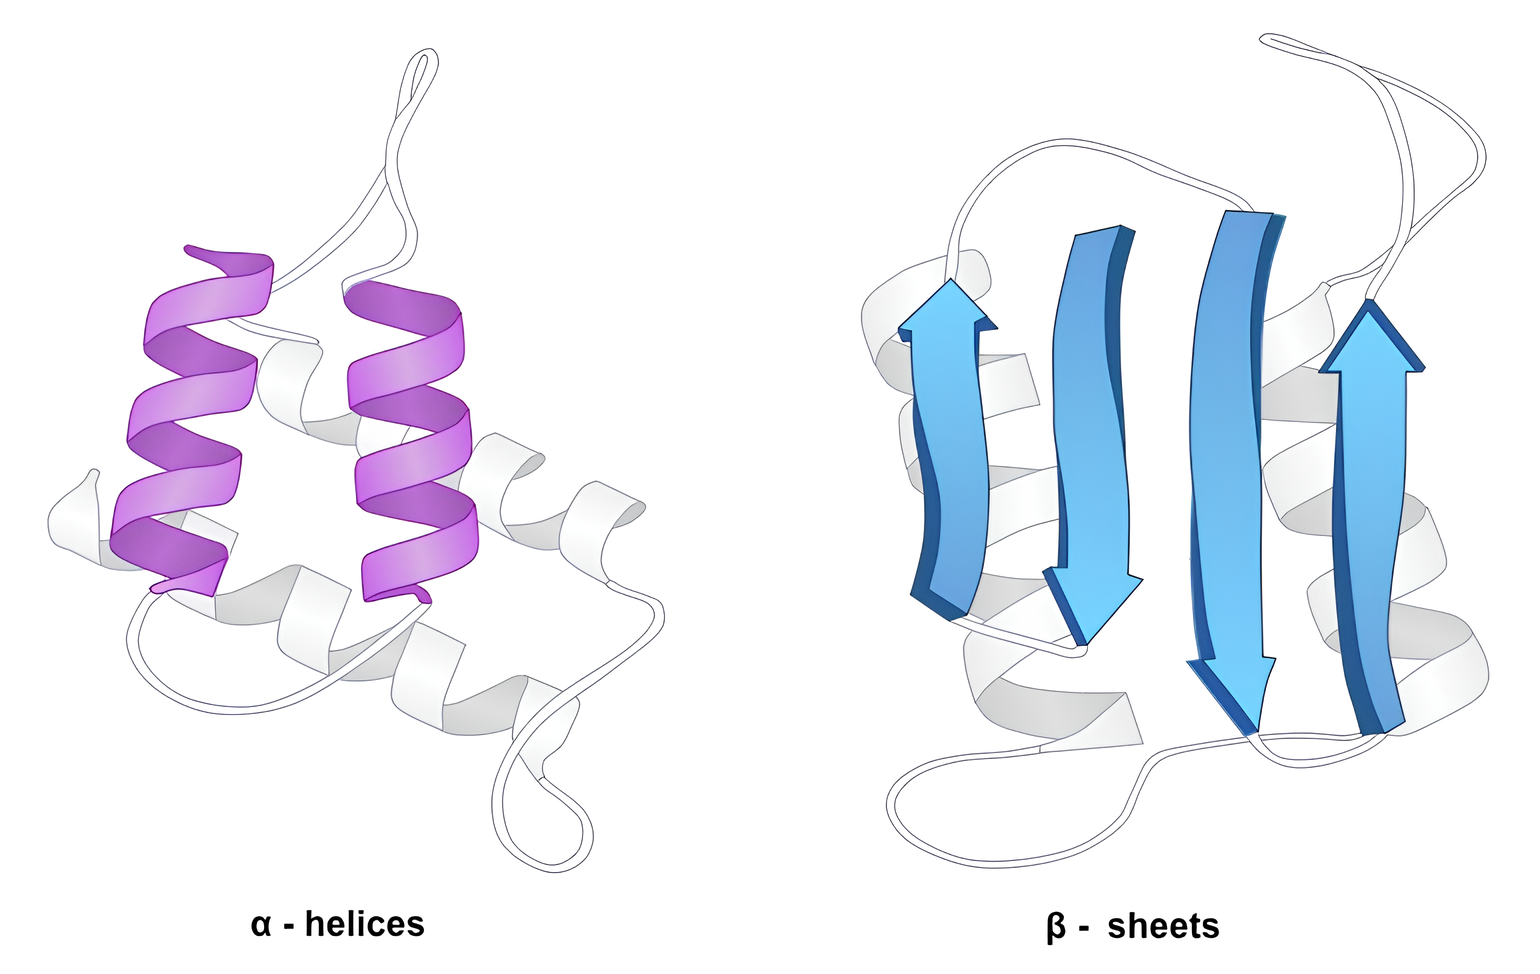
\includegraphics[width=0.8\textwidth]{img/ah_bs.png}
    \caption{Illustration of an alpha helix and a beta sheet, the two most common types of protein secondary structure. Generated with DALL·E 3.}
    \label{fig:alpha-beta}
\end{figure}

\xxx{TODO: change the picture}

The second level of protein structure is the \textbf{secondary structure}, which refers to local folding patterns within the polypeptide chain. The most common secondary structures are \textbf{alpha helices} and \textbf{beta sheets}, as shown in Figure~\ref{fig:alpha-beta}. These structures arise from hydrogen bonding between the backbone atoms of the amino acids, stabilizing the overall protein structure. All proteins also have a \textbf{three-dimensional (3D) structure}, also known as \textbf{tertiary structure}, which is crucial for their function \cite{nelson2008lehninger}, \cite{voet2010biochemistry}.

The secondary and tertiary structures are determined by the interactions between the side chains of the amino acids, including hydrophobic interactions, hydrogen bonds, ionic bonds, and disulfide bridges. The final level of protein structure is the \textbf{quaternary structure}, which refers to the assembly of multiple polypeptide chains into a functional protein complex \cite{nelson2008lehninger}, \cite{voet2010biochemistry}.

The tertiary and quaternary structures of proteins are determined through experimental methods such as X-ray crystallography and nuclear magnetic resonance (NMR) spectroscopy \cite{berman2000protein}. However, with the rise of deep learning and artificial intelligence, it is now also possible to predict protein structures from their amino acid sequences with remarkable accuracy. The most notable example is AlphaFold \cite{jumper2021highly}, \cite{abramson2024accurate}, a deep learning model developed by DeepMind that has achieved remarkable accuracy in predicting protein structures and has been widely adopted in the field of bioinformatics. AlphaFold also provides a per-residue confidence metric called the predicted Local Distance Difference Test (plDDT) score\footnotemark[1], which indicates the reliability of the predicted atomic positions. In recognition of the profound impact of these advances, the Nobel Prize in Chemistry was awarded in 2024 for the development of methods for the prediction of protein structures using artificial intelligence \cite{abriata2024nobel}. Other notable tools introduced in the past months include Boltz-2 \cite{passaro2025boltz2} and Chai-1 \cite{chai2024chai}. Today, predicted structures often closely match experimental results, as illustrated in Figure~\ref{fig:alphafold-vs-exp}.

\footnotetext[1]{The predicted Local Distance Difference Test (plDDT) score is a per-residue confidence metric output by AlphaFold, indicating the reliability of the predicted atomic positions; higher values suggest greater confidence. In the color scheme, blue indicates the most confident regions, while orange/yellow depict less confident regions.}

\begin{figure}[ht]
    \centering
    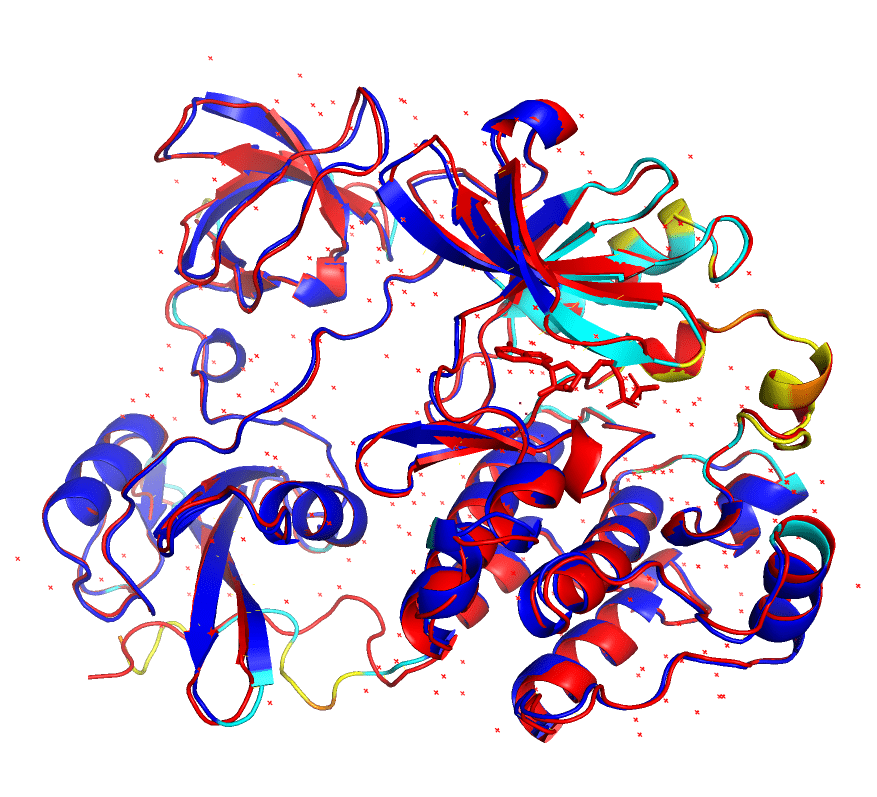
\includegraphics[width=0.8\textwidth]{img/alphafold_vs_exp.png}
    \caption{Comparison of AlphaFold predicted structure and experimental structure of the protein 2SRC (Crystal Structure of Human Tyrosine-Protein Kinase C-SRC, in Complex with AMP-PNP). The predicted structure is shown in blue to yellow colors (depicting the plDDT score), while the experimental structure is shown in red. The two structures are nearly identical after the alignment, demonstrating the accuracy of AlphaFold predictions. Image created in PyMOL.}
    \label{fig:alphafold-vs-exp}
\end{figure}
\par

Protein function is largely determined by interactions with other molecules, known as ligands. These may be small molecules, ions, RNA molecules, lipids, saccharides, or other molecules that bind to specific regions, often resulting in conformational changes that lead to different functions. Such interactions are crucial for processes like enzymatic catalysis, signal transduction, and immune response. In drug discovery, identifying and characterizing these sites is important, with computational approaches aiding both new therapeutic development and drug repurposing \cite{konc2019binding}. Additionally, de novo protein design allows for the creation of proteins with tailored functions, often guided by predictive tools such as AlphaFold before experimental testing \cite{huang2016coming}.

\section{Cryptic Binding Sites (CBSs)}
\label{sec:binding-sites}

\textbf{Binding sites} are distinct regions on a protein where ligands can bind and interact. These sites typically manifest as cavities or grooves on the protein surface and are frequently linked to conformational changes that influence protein function. Proteins with a ligand bound are termed \textbf{holo} conformations, while those lacking a ligand are called \textbf{apo} conformations. In holo conformations, the binding site is defined by the ligand’s position, whereas apo conformations may contain several potential binding sites, also commonly known as \textbf{pockets}.

\textbf{Cryptic binding sites (CBSs)} are regions on proteins that are not visible or accessible in the unbound (apo) structure but can form and become available for ligand binding following conformational changes. These sites typically appear only after ligand interaction or other molecular events that induce structural rearrangements. Computational methods such as CryptoBench \cite{vskrhak2025cryptobench} have been created to predict cryptic binding sites. A significant contribution in this area is CryptoSite \cite{cimermancic2016cryptosite}, which leverages known apo-holo protein pairs to identify CBSs, offering an alternative to time-consuming molecular dynamics simulations. Both of the methods will be covered in more detail in Section~\ref{sec:related-tools}.

\section{Databases and File Formats}
\label{sec:dbs-formats}

This section provides an overview of the key bioinformatics databases for protein structures and introduces the main file formats used in this field.

\subsection{PDB Archive and RCSB PDB}
\label{sec:rcsb-pdb}

The PDB (Protein Data Bank) Archive, often referred to simply as the "PDB database", is a comprehensive repository of 3D structural data for experimentally determined proteins, nucleic acids, and complex assemblies. It serves as a foundational resource for bioinformatics, with many machine learning and deep learning models relying on its data for training and validation. The archive is maintained by the wwPDB (Worldwide PDB) organization \cite{berman2003announcing}, which includes the RCSB PDB (Research Collaboratory for Structural Bioinformatics Protein Data Bank) \cite{berman2000protein}, PDBe (Protein Data Bank in Europe) \cite{velankar2010pdbe}, PDBj (Protein Data Bank Japan) \cite{kinjo2012protein}, and other members. 

The RCSB PDB (Research Collaboratory for Structural Bioinformatics Protein Data Bank) group offers a REST API for programmatic data access, which is publicly accessible at \url{https://www.rcsb.org/}. As of June 2025, the database contains over 238,000 structures.

Many organizations also maintain local, enriched copies of the PDB archive. The open sharing of structural data is encouraged, as it supports the development and improvement of computational models used throughout the scientific community \cite{callaway2025alphafold}.

\subsection{AlphaFold Database}
\label{sec:alphafold-db}

The AlphaFold Database \cite{varadi2024alphafold} contains over 200 million protein structures predicted by the AlphaFold model. While the majority of these structures have not been experimentally validated, those with high pLDDT scores are considered reliable. It is important to note that certain protein regions, known as intrinsically disordered regions, may exhibit low pLDDT scores due to their inherent flexibility and lack of stable structure. The database is publicly available at \url{https://alphafold.ebi.ac.uk/}.

\subsection{UniProt Database}
\label{sec:uniprot-db}

The UniProt database \cite{uniprot2025uniprot} is a comprehensive resource for protein sequences and functional information. Each protein is assigned a unique \textbf{UniProt accession} (also called \textbf{protein ID}), which serves as a standardized identifier for that specific protein. A single UniProt accession may correspond to multiple experimental structures in the PDB database, representing different conformations or states of the same protein, while typically having one predicted structure in the AlphaFold database. UniProt accessions are commonly used to link PDB and AlphaFold entries. UniProt is available at \url{https://www.uniprot.org/}. The main part of the UniProt database is the UniProt Knowledgebase (UniProtKB), which contains two sections: UniProtKB/Swiss-Prot, which includes manually curated entries with high-quality annotations, and UniProtKB/TrEMBL, which contains automatically annotated entries that have not yet been reviewed \cite{boutet2016uniprotkb}.

\subsection{PDB File Format}
\label{sec:pdb-format}

The PDB (Protein Data Bank) file format is a text-based format used to represent three-dimensional structures of biological molecules, primarily proteins and nucleic acids. It contains information about atom coordinates, connectivity, b-factors, and other structural details. Each PDB file should start with header lines providing metadata about the structure, such as the structure name, authors, methods used and additional comments. Then, the atomic coordinates are listed in a list of ATOM and HETATM records, which specify the atom type, residue name, chain identifier, residue sequence number, and the x, y, z coordinates of each atom in the structure. The PDB format might include information about secondary structure elements, such as helices and sheets \cite{westbrook2003pdb}. Some of the information might be ommited, especially in the case of working with structures generated by deep learning methods, such as RFDiffusion \cite{watson2023novo}. A single PDB file may contain multiple models representing distinct conformations of the same protein. It is worth noting that the PDB format is considered deprecated in favor of the more modern mmCIF format (covered in \ref{sec:mmcif-format}), though it remains widely used due to its simplicity and broad tool support.

\begin{figure}[H]
    \centering
    \lstinputlisting[caption={
        An edited example of a PDB file containing information about a protein structure generated by RFDiffusion.
    }]{code/rfdiff_example.pdb}
\end{figure}


\subsection{mmCIF File Format}
\label{sec:mmcif-format}

The mmCIF (Macromolecular Crystallographic Information File, also called PDBx) format is a more modern and flexible alternative to the PDB format, designed to overcome the limitations of the PDB format, especially for large structures \cite{bourne199730}. The PDB database, mentioned in Section~\ref{sec:rcsb-pdb}, has been transitioning to the mmCIF format for new entries. Although it is encouraged to use mmCIF for new structures, many existing tools and databases still rely on the PDB format thanks to its simpler format. Like PDB files, mmCIF files can also represent multiple conformations of the same structure.

\subsection{FASTA File Format}
\label{sec:fasta-format}

The FASTA file format is a widely used, text-based format for representing biological sequences, such as proteins or nucleic acids. Each sequence entry begins with a header line that starts with a ">" character, followed by a description or identifier. The sequence itself is written on the following lines, typically using single-letter codes. Multiple sequences can be included in a single FASTA file, each with its own header. While the header line is commonly present, it is technically optional, which allows easy creation of FASTA files \cite{lipman1985rapid}.

\begin{figure}[H]
    \centering
    \lstinputlisting[
        caption={
            An example of a FASTA file containing information about the 6A5J sequence (containing only 13 amino acids).
        },
        breaklines=true
    ]{code/fasta_example.fasta}
\end{figure}

\section{Related Tools, Projects}
\label{sec:related-tools}

This section is dedicated to the most relevant tools and projects important for the work presented in this thesis.

\subsection{P2Rank, PrankWeb}
\label{sec:prankweb-p2rank}

P2Rank is a Groovy/Java based standalone tool for predicting binding sites in protein structures. The P2Rank algorithm is based on machine learning. The structure is covered with a grid of points on the protein's solvent accessible surface, and each point is assigned a score based on the likelihood of being a binding site based on the local environment of the point. Then, the points are clustered and ranked based on their scores. The pre-trained tool does not rely on any external databases nor templates. The method is widely adapted due to its reliable and accurate predictions and speed \cite{krivak2018p2rank}. Source codes for P2Rank are available at \url{https://github.com/rdk/p2rank}.

PrankWeb is a web-based interface for P2Rank, allowing simple access to the P2Rank method without the need to run and install the tool locally. It is available at \url{https://prankweb.cz/}. The web interface allows users to upload a PDB/mmCIF file and receive a visualization of the prediction of the binding sites with the predicted binding sites colored according to their scores. Moreover, PrankWeb allows the users to perform molecular docking using the predicted binding sites, which is a common post-processing step in drug discovery \cite{polak2025prankweb}, \cite{jakubec2022prankweb}, \cite{jendele2019prankweb}. The docking is performed using the AutoDock Vina \cite{trott2010autodock} software, which is a widely used tool for molecular docking.

The PrankWeb interface was a huge inspiration for the design of the web interface presented in this thesis as the goal is to provide a similar user experience, but with a focus on cryptic binding sites and its specific challenges.

\subsection{AHoJ}
\label{sec:ahoj}

AHoJ (Apo–Holo Juxtaposition) is a web application for retreiving and visualizing apo-holo pairs of proteins (See Section~\ref{sec:binding-sites}). This functionality is useful especially for cryptic binding site predictions, as it allows the users to find similar structures with possibly similar properties based on the predicted CBS \cite{feidakis2022ahoj}. The application is available at \url{https://apoholo.cz/}. Currently, AHoJ supports searching for apo-holo pairs only by PDB ID.

AHoJ is integrated within the CryptoShow interface as well. This will be covered in more detail in Section~\ref{sec:trajectory}.

\subsection{PyMOL}
\label{sec:pymol}

PyMOL is a powerful molecular visualization tool written in Python. The users might use it either as a standalone application or as a Python library. Thanks to its feature-rich API and UI, PyMOL is a common choice for researchers in structural biology and cheminformatics \cite{delano2002pymol}.

\subsection{Mol*}
\label{sec:molstar}

Mol* (also MolStar) is a TypeScript library for visualizing molecular structures directly in web browsers. Thanks to its modern architecture, the usage of WebGL and rich feature set, Mol* is nowadays a very popular choice for web-based molecular visualization tools \cite{sehnal2018mol}. Mol* also provides an online version of a molecular viewer, which is available at \url{https://molstar.org/viewer/} \cite{sehnal2021mol}. A highly-customized version of the viewer is also used in the CryptoShow interface, which will be covered in more detail in Section~\ref{sec:frontend-molstar}.

\begin{figure}[ht]
    \centering
    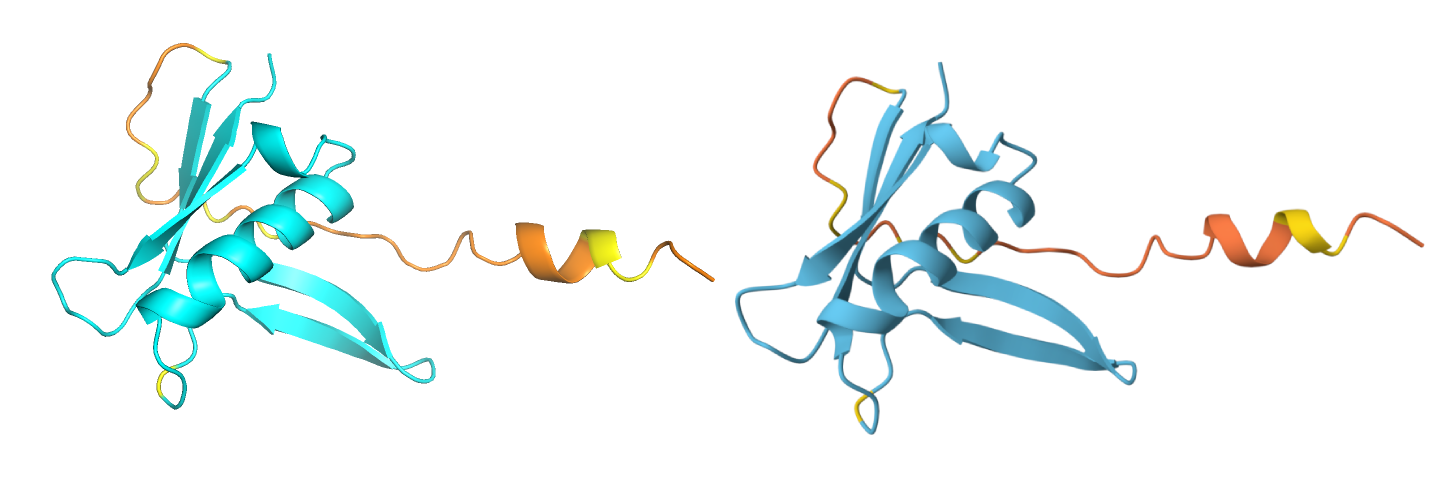
\includegraphics[width=\textwidth]{img/pymol-molstar.png}
    \caption{A comparsion of the PyMOL (left) and Mol* (right) molecular viewers showing the AlphaFold predicted structure of the protein AF\_AFQ9XWU9F1.}
    \label{fig:pymol-molstar}
\end{figure}

\subsection{CryptoBench}
\label{sec:cryptobench}

CryptoBench is a comprehensive benchmark dataset for training and evaluating CBSs prediction methods, built from a large set of apo–holo protein pairs and grouped by UniProt ID with predefined cross-validation splits. A part of the publication is dedicated to baseline evaluations, which show that a sequence-based neural network using protein language model embeddings outperforms state-of-the-art structure-based methods like PocketMiner \cite{meller2023predicting} and P2Rank \cite{krivak2018p2rank} across key metrics in terms of CBSs. The source codes for CryptoBench are available at \url{https://github.com/skrhakv/CryptoBench/} \cite{vskrhak2025cryptobench}.

The model used in CryptoBench (referred to as \textbf{CB-Model} in the context of this thesis) is able to predict cryptic binding sites when provided with ESM-2 embeddings \cite{lin2022language} of the protein sequence. The prediction capability represents one of the core functionalities of CryptoShow. More details about the CryptoBench method will be provided in Section~\ref{sec:prediction}.

\subsection{CryptoSite}
\label{sec:cryptosite}

CryptoSite is another tool designed to identify CBSs. By constructing a dataset of structurally defined apo–holo pairs, CryptoSite characterizes cryptic sites based on sequence, structure, and dynamics. Leveraging these insights, CryptoSite uses machine learning to predict cryptic sites with high accuracy, expanding the set of potentially druggable proteins. The tool has been applied to the human proteome, increasing the fraction of disease-associated proteins considered druggable. Experimental validation further demonstrates the practical use of CryptoSite. The web server is accessible at \url{https://modbase.compbio.ucsf.edu/cryptosite} \cite{cimermancic2016cryptosite}.

While CryptoSite is a valuable resource for cryptic binding site analysis and its web server remains available, its computational processes often take several days to complete, limiting its suitability for interactive use. In contrast, a primary goal of CryptoShow is to provide a fast and interactive experience, allowing users to obtain results within minutes. This need is underscored by the relatively low usage of CryptoSite; as of June 2025, only 10 jobs were submitted in the last 7 days. Also, the results of the CryptoSite jobs are available only for 7 days after the job completion.

\chapter{Methodology}
\label{chap:methodology}

In this chapter, we will cover the methodology used in this work. More details on the pipeline execution will be provided in Section \ref{sec:backend}.

\section{Prediction Using the CryptoBench Model, ESM-2}
\label{sec:prediction}

The initial step in our methodology involves utilizing the CryptoBench \cite{vskrhak2025cryptobench} model to generate residue-level predictions for protein sequences. It is important to note that this model works solely with sequence information, without incorporating any structural (tertiary or quaternary) data. Specifically, we employ the tiny variant of CryptoBench\footnote{Available at \url{https://github.com/skrhakv/TinyCryptobench}}, which is trained on a reduced version of the fine-tuned ESM-2 embeddings \cite{lin2022language} with 650 million parameters, as opposed to the full 3 billion. This choice is motivated by the observation that prediction accuracy remains comparable, while computational requirements are significantly reduced, enabling the pipeline to run efficiently on standard personal computers without the need for a GPU.

CryptoBench was created by filtering the AHoJ-DB \cite{feidakis2024ahoj} dataset, which contains a few million binding pockets. The filtering steps involved resolution filtering, removing redundant structures, geometric quality assurance, crypticity constraints, ligand filtering and sequence clustering. The final dataset consists of 1107 apo structures with 1361 cryptic binding sites. This dataset is used to train the model that has been benchmarked against PocketMiner \cite{meller2023predicting} and P2Rank \cite{krivak2018p2rank} and has shown better performance with the apo structures.

\sloppy
To begin with the prediction, the necessary dependencies for the CryptoBench model must be installed. Once the Python environment is set up, the fine-tuned ESM-2 model (\lstinline!facebook/esm2_t33_650M_UR50D!) is loaded, followed by the corresponding weight file from the Tiny-CryptoBench repository. The protein sequence is then tokenized using the ESM-2 tokenizer, segmented into chunks of 1022 tokens (1024 minus two special tokens), and processed by the CryptoBench model to obtain predictions. These predictions are subsequently concatenated to produce a single prediction vector representing the entire sequence.

\sloppy
The implementation for this procedure is provided in the \lstinline!backend/prediction/compute_score.py! file. The code is intended for use with individual protein sequences, as it requires parsing and splitting the sequence by chain to ensure accurate predictions.

This code is run asynchronously using Celery workers, allowing efficient processing of multiple sequences in parallel. Moreover, the implementation supports both GPU and CPU execution.

After the predictions are generated, the next step is to look for potential clusters of high-scoring residues and create the corresponding binding site candidates, as described in Section~\ref{sec:clustering}.

\section{Clustering and Smoothing}
\label{sec:clustering}

\xxx{TODO}

\section{Trajectory Animation}
\label{sec:trajectory}

\xxx{TODO}

\chapter{Software}
\label{chap:software}

The third chapter of this thesis describes the web application, CryptoShow, which is developed to provide a user-friendly interface for the methodology described in Chapter~\ref{chap:methodology}. This chapter covers the architecture, technologies used, backend and frontend development, testing, monitoring, and deployment of the application.

\section{Architecture and Used Technologies}
\label{sec:architecture-technologies}

This section outlines the architecture of the CryptoShow application and the technologies employed in its development. The application is designed to be modular and scalable, allowing for easy integration of new features and improvements. For this purpose, we have chosen a service-oritented architecture (SOA) that separates the components, enabling independent development and deployment. The architecture is defined by several Docker containers\footnote{Available at \url{https://www.docker.com/}.}, each responsible for a specific part of the application. The services are orchestrated using Docker Compose, defined in the \texttt{docker-compose.yml} file, which specifies the services, networks, and volumes required for the application to run. The service architecture is as follows:

\begin{itemize}
    \item \textbf{backend} - Acts as the central API service, facilitating communication between most components. It communicates with Redis\footnote{Available at \url{https://redis.io/}.}, manages API requests from the frontend, and delegates asynchronous tasks to Celery workers\footnote{Available at \url{https://github.com/celery/celery}.}. The FastAPI server\footnote{Available at \url{https://github.com/fastapi/fastapi}.} serves as its entry point. Further details are provided in Section~\ref{sec:backend}.
    \item \textbf{worker-cpu / worker-gpu} - These two services execute asynchronous, resource-intensive computational tasks (i.e. the prediction, smoothing, and trajectory animation) without blocking the main FastAPI event loop. \texttt{worker-cpu} runs on the CPU, while \texttt{worker-gpu} leverages GPU acceleration via CUDA when available. More details are provided in Section~\ref{sec:backend}.
    \item \textbf{frontend} - Delivers the user interface. NginX\footnote{Available at \url{https://nginx.org/}.} acts as the gateway to the defined services in Docker Compose and serves static content from a specified directory. Additional information is available in Section~\ref{sec:frontend}.
    \item \textbf{redis} - Functions as the message broker for Celery workers, enabling efficient task distribution.
    \item \textbf{monitoring-flag} - A minimal service that generates a flag file to activate the monitoring proxy endpoint. Additional information about this service and those that follow is available in Section~\ref{sec:tests-monitoring}.
    \item \textbf{remove-monitoring-flag} - A lightweight service that removes the monitoring flag file, disabling the monitoring endpoint.
    \item \textbf{flower\footnote{Available at \url{https://github.com/mher/flower}.}} - Provides real-time monitoring and statistics for Celery tasks and queues.
    \item \textbf{celery-exporter\footnote{Available at \url{https://github.com/danihodovic/celery-exporter}.}} - Exposes Celery metrics to Prometheus, similarly to the Flower service.
    \item \textbf{prometheus\footnote{Available at \url{https://prometheus.io/}.}} - Collects and stores metrics exported from the Celery workers.
    \item \textbf{grafana\footnote{Available at \url{https://grafana.com/}.}} - Offers a user-friendly dashboard for visualizing metrics collected by Prometheus.
\end{itemize}

\begin{figure}[htpb]
    \centering
    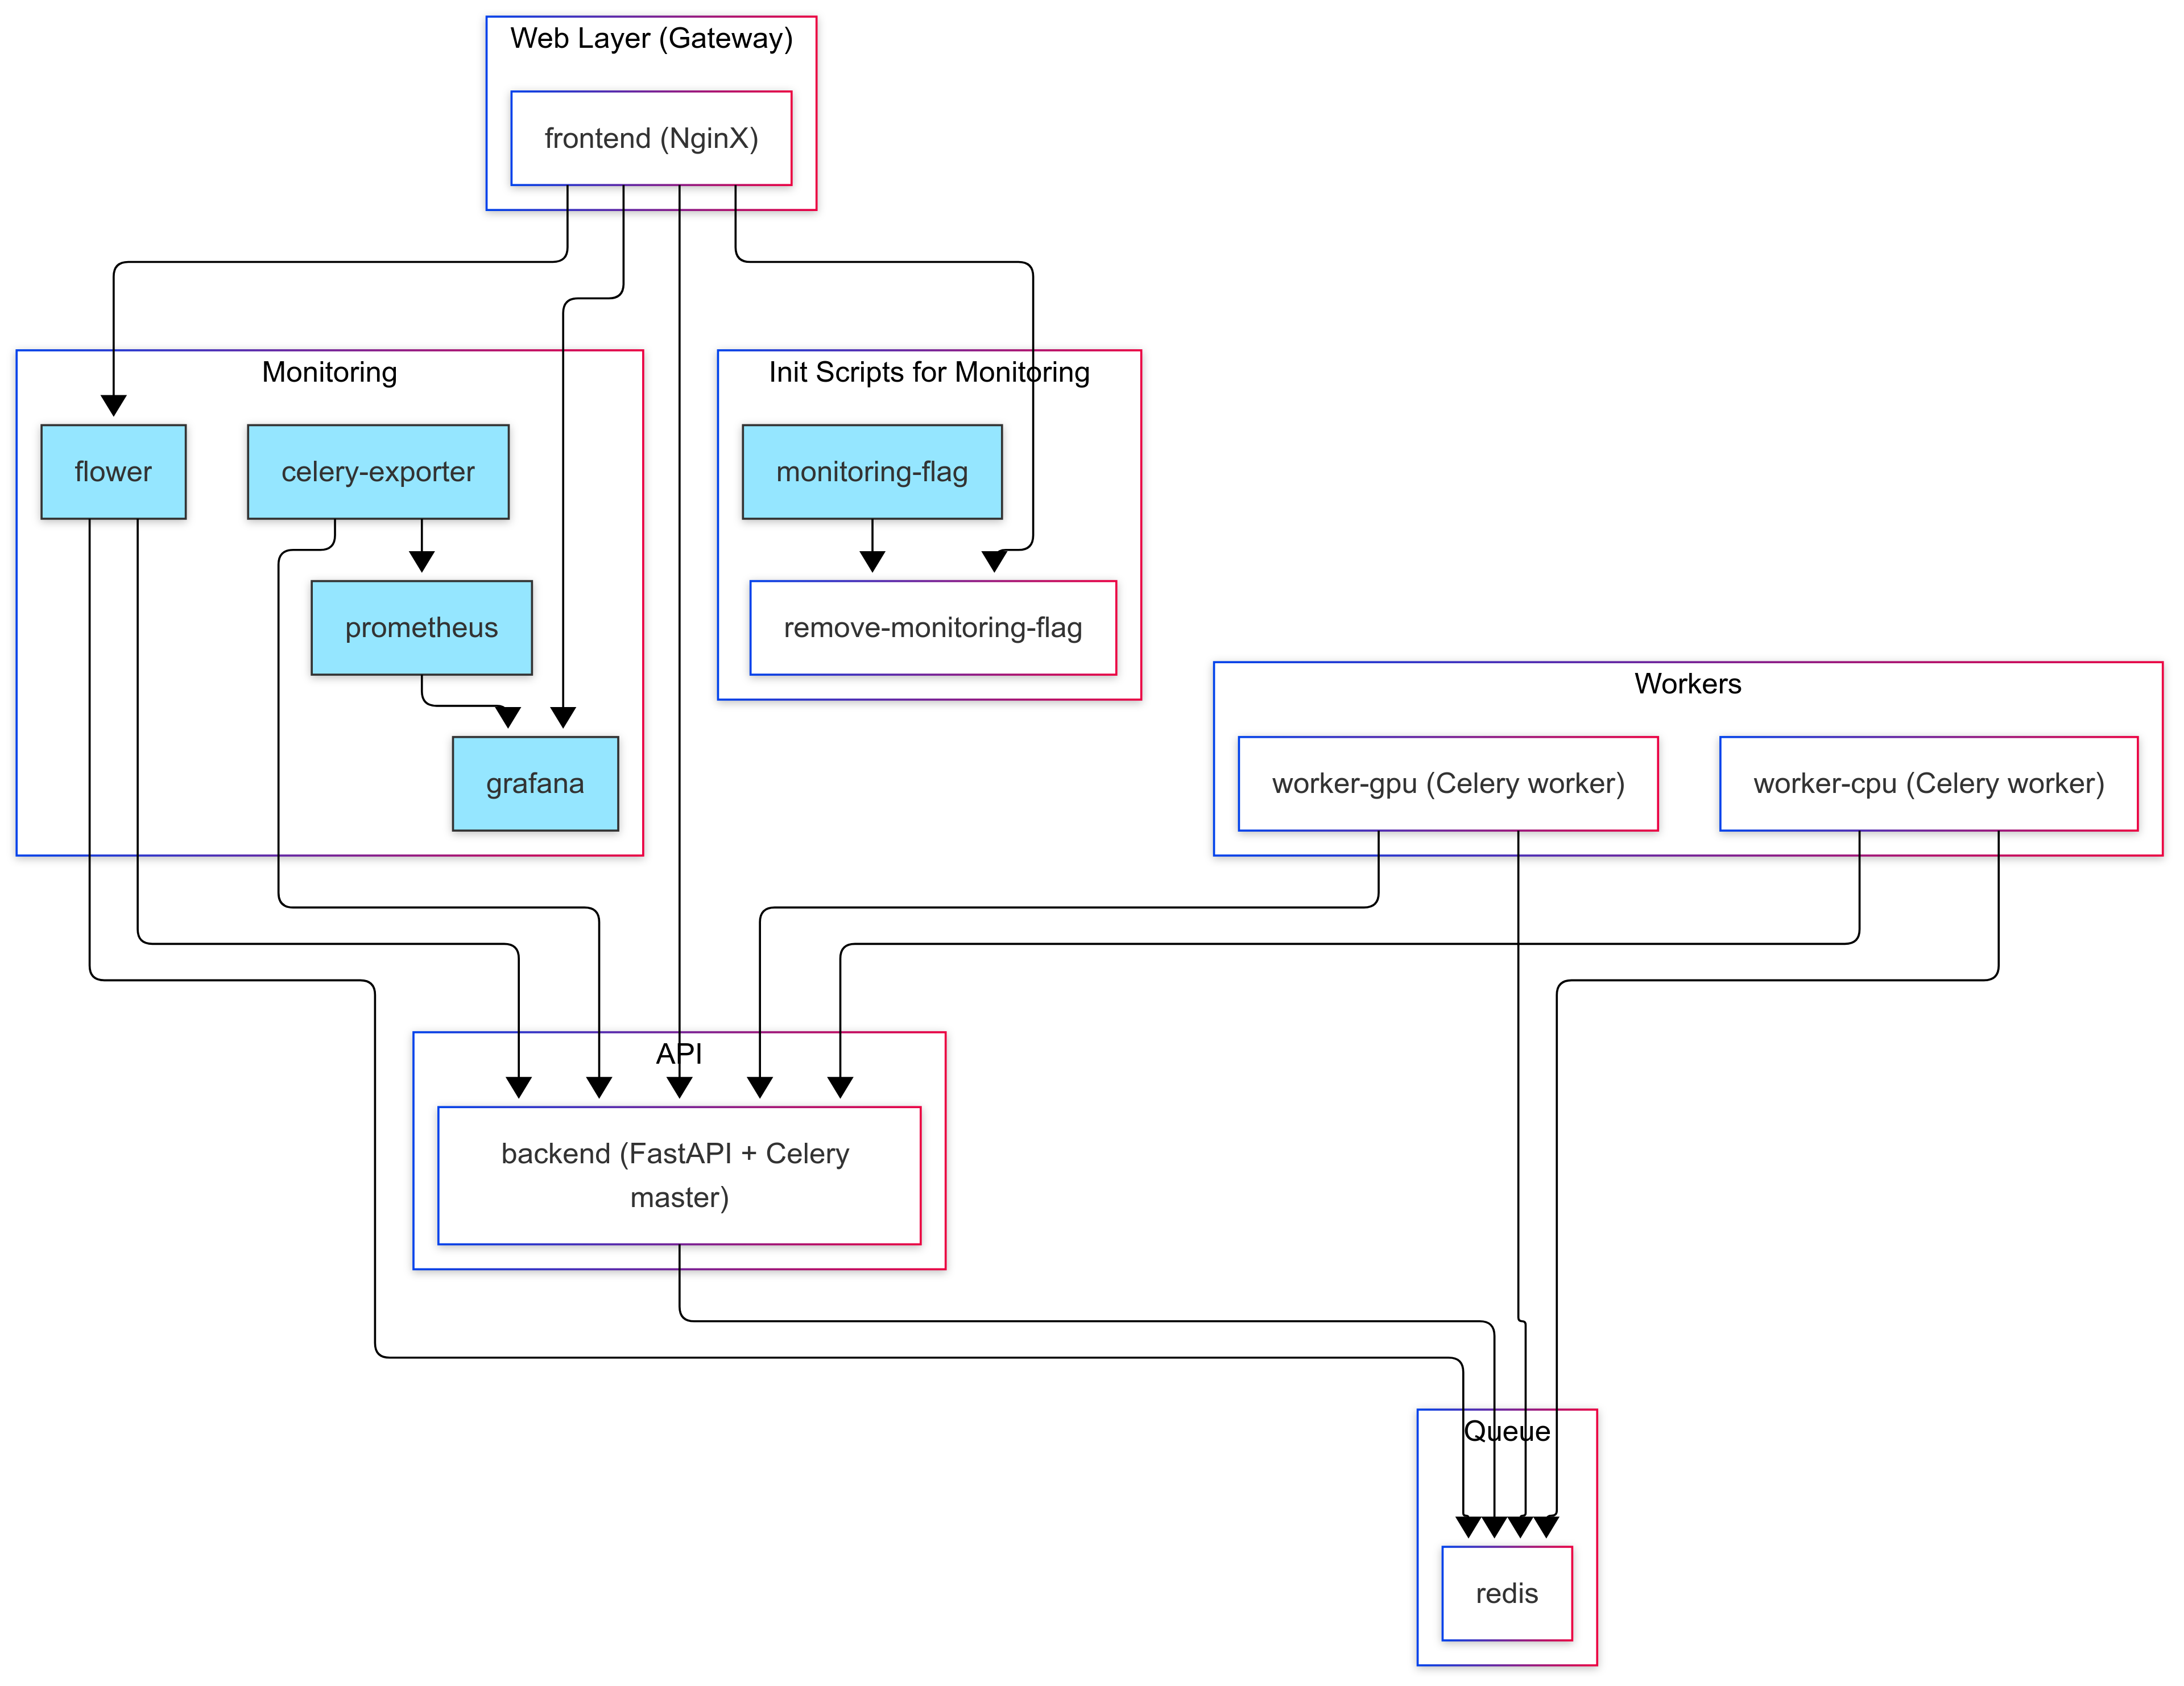
\includegraphics[width=\textwidth]{img/architecture.png}
    \caption{Service architecture of the CryptoShow application. Each small box represents a Docker containerized service. Light blue services are optional, as monitoring is not always required. Arrows indicate communication paths between services. Generated using the Mermaid Chart tool, available at \url{https://www.mermaidchart.com/}.}
    \label{fig:architecture}
\end{figure}

An overview of the service architecture can be seen in Figure~\ref{fig:architecture}. This type of architecture offers a scalable solution that has the potential of easy deployment and development.

Let's also focus on the technology stack for some of the services:

\begin{itemize}
    \item \textbf{backend, worker-cpu / worker-gpu} - Python, notable libraries and tools: Celery (asynchronous tasks in Python), FastAPI, Flower, PyTorch, BioPython, Biotite, Scikit-Learn, MDAnalysis, Gemmi, Redis, uv
    \item \textbf{frontend} - TypeScript, notable libraries, tools and frameworks: React, NginX, Mol*, Bun, Vite
\end{itemize}

The remaining services utilize standard technology stacks commonly associated with their respective functionalities.

\section{Backend}
\label{sec:backend}

The backend of the CryptoShow application is responsible for the core functionalities, such as calculating the predictions, clustering and smoothing the results, generating trajectory animations for AHoJ results, and serving the API endpoints for the frontend. This section covers the \textbf{backend, worker-cpu, worker-gpu} and \textbf{redis} services. All source codes can be found in the \lstinline!backend! directory.

All backend services utilize the same initial Dockerfile with one Python environment. This ensures consistency and speeds up the build process. For the installation of the Python environment, we use the \lstinline!pyproject.toml! file, which contains all necessary dependencies for the backend services, and is installed using the \lstinline|uv| tool\footnote{Available at \url{https://github.com/astral-sh/uv}.}. After installing the Python environment, the entrypoint for the backend service is run, which first checks for the presence of the machine learning models and downloads them if they are not available. Subsequently, the FastAPI server is started running on port 5000.

\subsection{FastAPI}
\label{sec:fastapi}

The backend service is built using FastAPI, a modern web framework for building APIs with Python. It serves as the main entry point for the application, handling API requests and delegating tasks to Celery workers.

FastAPI is chosen for its performance and ease of use, including the option to automatically generate OpenAPI documentation (available via the \lstinline|/api/docs| endpoint). The server includes configuration for CORS (Cross-Origin Resource Sharing), logging and error handling. The API contains several endpoints, including endpoints for health check, prediction for a given PDB ID, prediction for a custom protein structure, Celery task status check, and trajectory animation generation. To improve performance, WebSockets are used to check the status of the tasks, allowing the frontend to receive updates without polling the server.

\xxx{TODO: include all API endpoints in the appendix}

To support asynchronous task execution without blocking the main event loop, the backend service uses Celery workers. These workers are responsible for executing resource-intensive tasks, such as running the CB-Model, smoothing model and generating trajectory animations. The workers can run on either CPU or GPU, depending on the availability of resources (covered in detail in \ref{sec:deployment}). The backend service communicates with Redis, which acts as a message broker for Celery, allowing efficient task distribution and management.

The logic for the API endpoints is implemented in the \lstinline!backend/main.py! file.

\subsection{Prediction and Clustering}
\label{sec:prediction-backend}

To begin with the prediction, the necessary dependencies for the CryptoBench model must be installed. Once the Python environment is set up (this is done in Docker automatically), the Celery task is added to the queue. The task is defined in the \lstinline!backend/tasks.py! file, which is responsible for executing the prediction logic.

First, the structure provided by the user (either in the form of an ID or a custom structure) is processed and parsed using specialized parsers for the PDB/mmCIF formats (see Section~\ref{sec:pdb-format} and Section~\ref{sec:mmcif-format}). Only the first model of the structure is considered, as the CryptoBench model is designed to work with single-model structures. After parsing, the structure is then converted to a protein sequence, saved to FASTA files (see Section~\ref{sec:fasta-format}) for each chain, which is required for the prediction.

Afterwards, the fine-tuned ESM-2 model (\lstinline!facebook/esm2_t33_650M_UR50D!\footnote{More information available at \url{https://github.com/facebookresearch/esm?tab=readme-ov-file#pre-trained-models-}.}) is loaded, followed by the corresponding weight file from the Tiny-CryptoBench repository. The protein sequence is then tokenized using the ESM-2 tokenizer, segmented into chunks of 1022 tokens (1024 minus two special tokens), and processed by the CryptoBench model to obtain predictions. These predictions are subsequently concatenated to produce a single prediction vector representing the entire sequence. The model consists of three linear layers, two dropout layers, and a ReLU activation function. Then, the predictions are generated by applying the sigmoid activation function to the output of the final linear layer, resulting in a vector of probabilities for each residue in the sequence. The implementation for this procedure is provided in the \lstinline!backend/prediction/compute_score.py! file. The code is intended for use with individual protein sequences, as it requires parsing and splitting the sequence by chain to ensure accurate predictions. Concatenating all chains into a single sequence would provide incorrect context to the model and result in inaccurate predictions.

After receiving the predictions for individual chains, 3D coordinates of all residues are extracted from the input structure. This step is required for the clustering and smoothing processes. The predictions are first clustered using the methodology described in Section~\ref{sec:clustering}. After clustering, the clusters are further smoothed. All source codes for the clustering and smoothing processes can be found in the \lstinline!backend/clustering! directory and follow the described methodology.

Following this refinement process, all collected data is collected into a single JSON object, which is subsequently stored, returned, and used by the frontend for result visualization.

\subsection{Trajectory Animation}
\label{sec:trajectory}

CryptoShow aims not only to predict and visualize cryptic binding sites, but also to demonstrate potential conformational changes through animated trajectories. To achieve this, we have developed a trajectory animation feature that illustrates structural transitions between related protein conformations.

Let us begin by introducing AHoJ \cite{feidakis2022ahoj} and AHoJ-DB \cite{feidakis2024ahoj} (briefly covered in Section \ref{sec:ahoj}). Apo–Holo Juxtaposition (AHoJ) is a web-based tool designed to identify apo-holo pairs of protein structures within the PDB database (Section~\ref{sec:rcsb-pdb}); currently, querying is limited to this database only.

AHoJ identifies binding residues by spatially marking user-defined ligands using PyMOL (Section~\ref{sec:pymol}). The typical workflow involves the user specifying a binding spot, either by selecting a ligand or defining a set of residues of interest in the query structure. The tool then searches for other structures of the same protein (i.e., structures sharing the same UniProt accession number, see Section~\ref{sec:uniprot-db}) that contain the same binding spot. It does this by mapping the binding residues onto the UniProt sequence and examining each candidate chain to determine whether the mapped binding residues are present above a minimum threshold. Successful candidates are aligned to the query chain using TM-align \cite{zhang2005tm}, and the area around the superimposed query ligand is examined for ligands. The process classifies each candidate chain as apo or holo based on ligand presence or absence in the defined binding sites, with results visualized in the browser and downloadable for PyMOL analysis. AHoJ-DB is a database of pre-computed apo-holo pairs of protein structures.

For CryptoShow's trajectory animation functionality, we make use of the AHoJ public API to identify apo-holo structural pairs corresponding to the input structure. The query process requires the PDB ID of the input structure\footnote{As mentioned above, AlphaFold structures and custom structures are not supported by AHoJ. Additionally, the input structure may be in holo form. This is not validated in any way. Apo structures are generally more appropriate for this analysis, we leave this decision on the user as it does not affect the functionality of CryptoShow.}, the target chain containing the predicted cryptic binding site, and the central residue of the identified CBS. Listing \ref{lst:ahoj-query} demonstrates the query format. The API response contains all available paired structures, from which users can select any structure to visualize potential conformational transitions. Upon selection, the CryptoShow API initiates the trajectory computation.

\begin{lstlisting}[caption={Sample query format for the AHoJ tool, specifying PDB ID 2src, chain A, aspartic acid residue at position 404}, label={lst:ahoj-query}]
    2src A ASP 404
\end{lstlisting}

First, the target structure for animation is downloaded from AHoJ. Then, combined with the original structure, both structure files are then converted to PDB format to ensure each contains only a single model and to allow easier manipulation compared to the mmCIF format (see Section~\ref{sec:pdb-format} and Section~\ref{sec:mmcif-format}). Subsequently, the PDB file is processed using the MDAnalysis library \cite{gowers2019mdanalysis}, from which the sequence and corresponding residues are extracted. At this point, we have obtained the necessary structural information.

Next, we need to determine which residues should be included in the animation. To achieve this, we employ a straightforward approach by computing the longest common subsequence of both protein sequences. This ensures that only residues present in both structures are animated. The subsequence length must be greater than zero due to the inherent logic of AHoJ. Once the common subsequence is identified, the corresponding residues from both structures are extracted. The MDAnalysis library is utilized to perform this operation at the atomic level, as PDB files store coordinates for individual atoms rather than residues. Additionally, all ligands are extracted from both structures to include them in the final animation.

In the end, the trajectory is generated using cubic spline interpolation \cite{mckinley1998cubic} implemented in the SciPy library \cite{virtanen2020scipy}. A trimmed PDB file containing only the relevant residues and ligands is created, along with a trajectory file \xxx{TODO: add trajectory file format} featuring interpolated coordinates across a predetermined number of frames (set arbitrarily to 50). The final visualization presents the original structure at 50\% opacity and the target holo structure at full opacity, as illustrated in Figure \ref{fig:trajectory-animation}.

\begin{figure}[htbp]
    \centering
    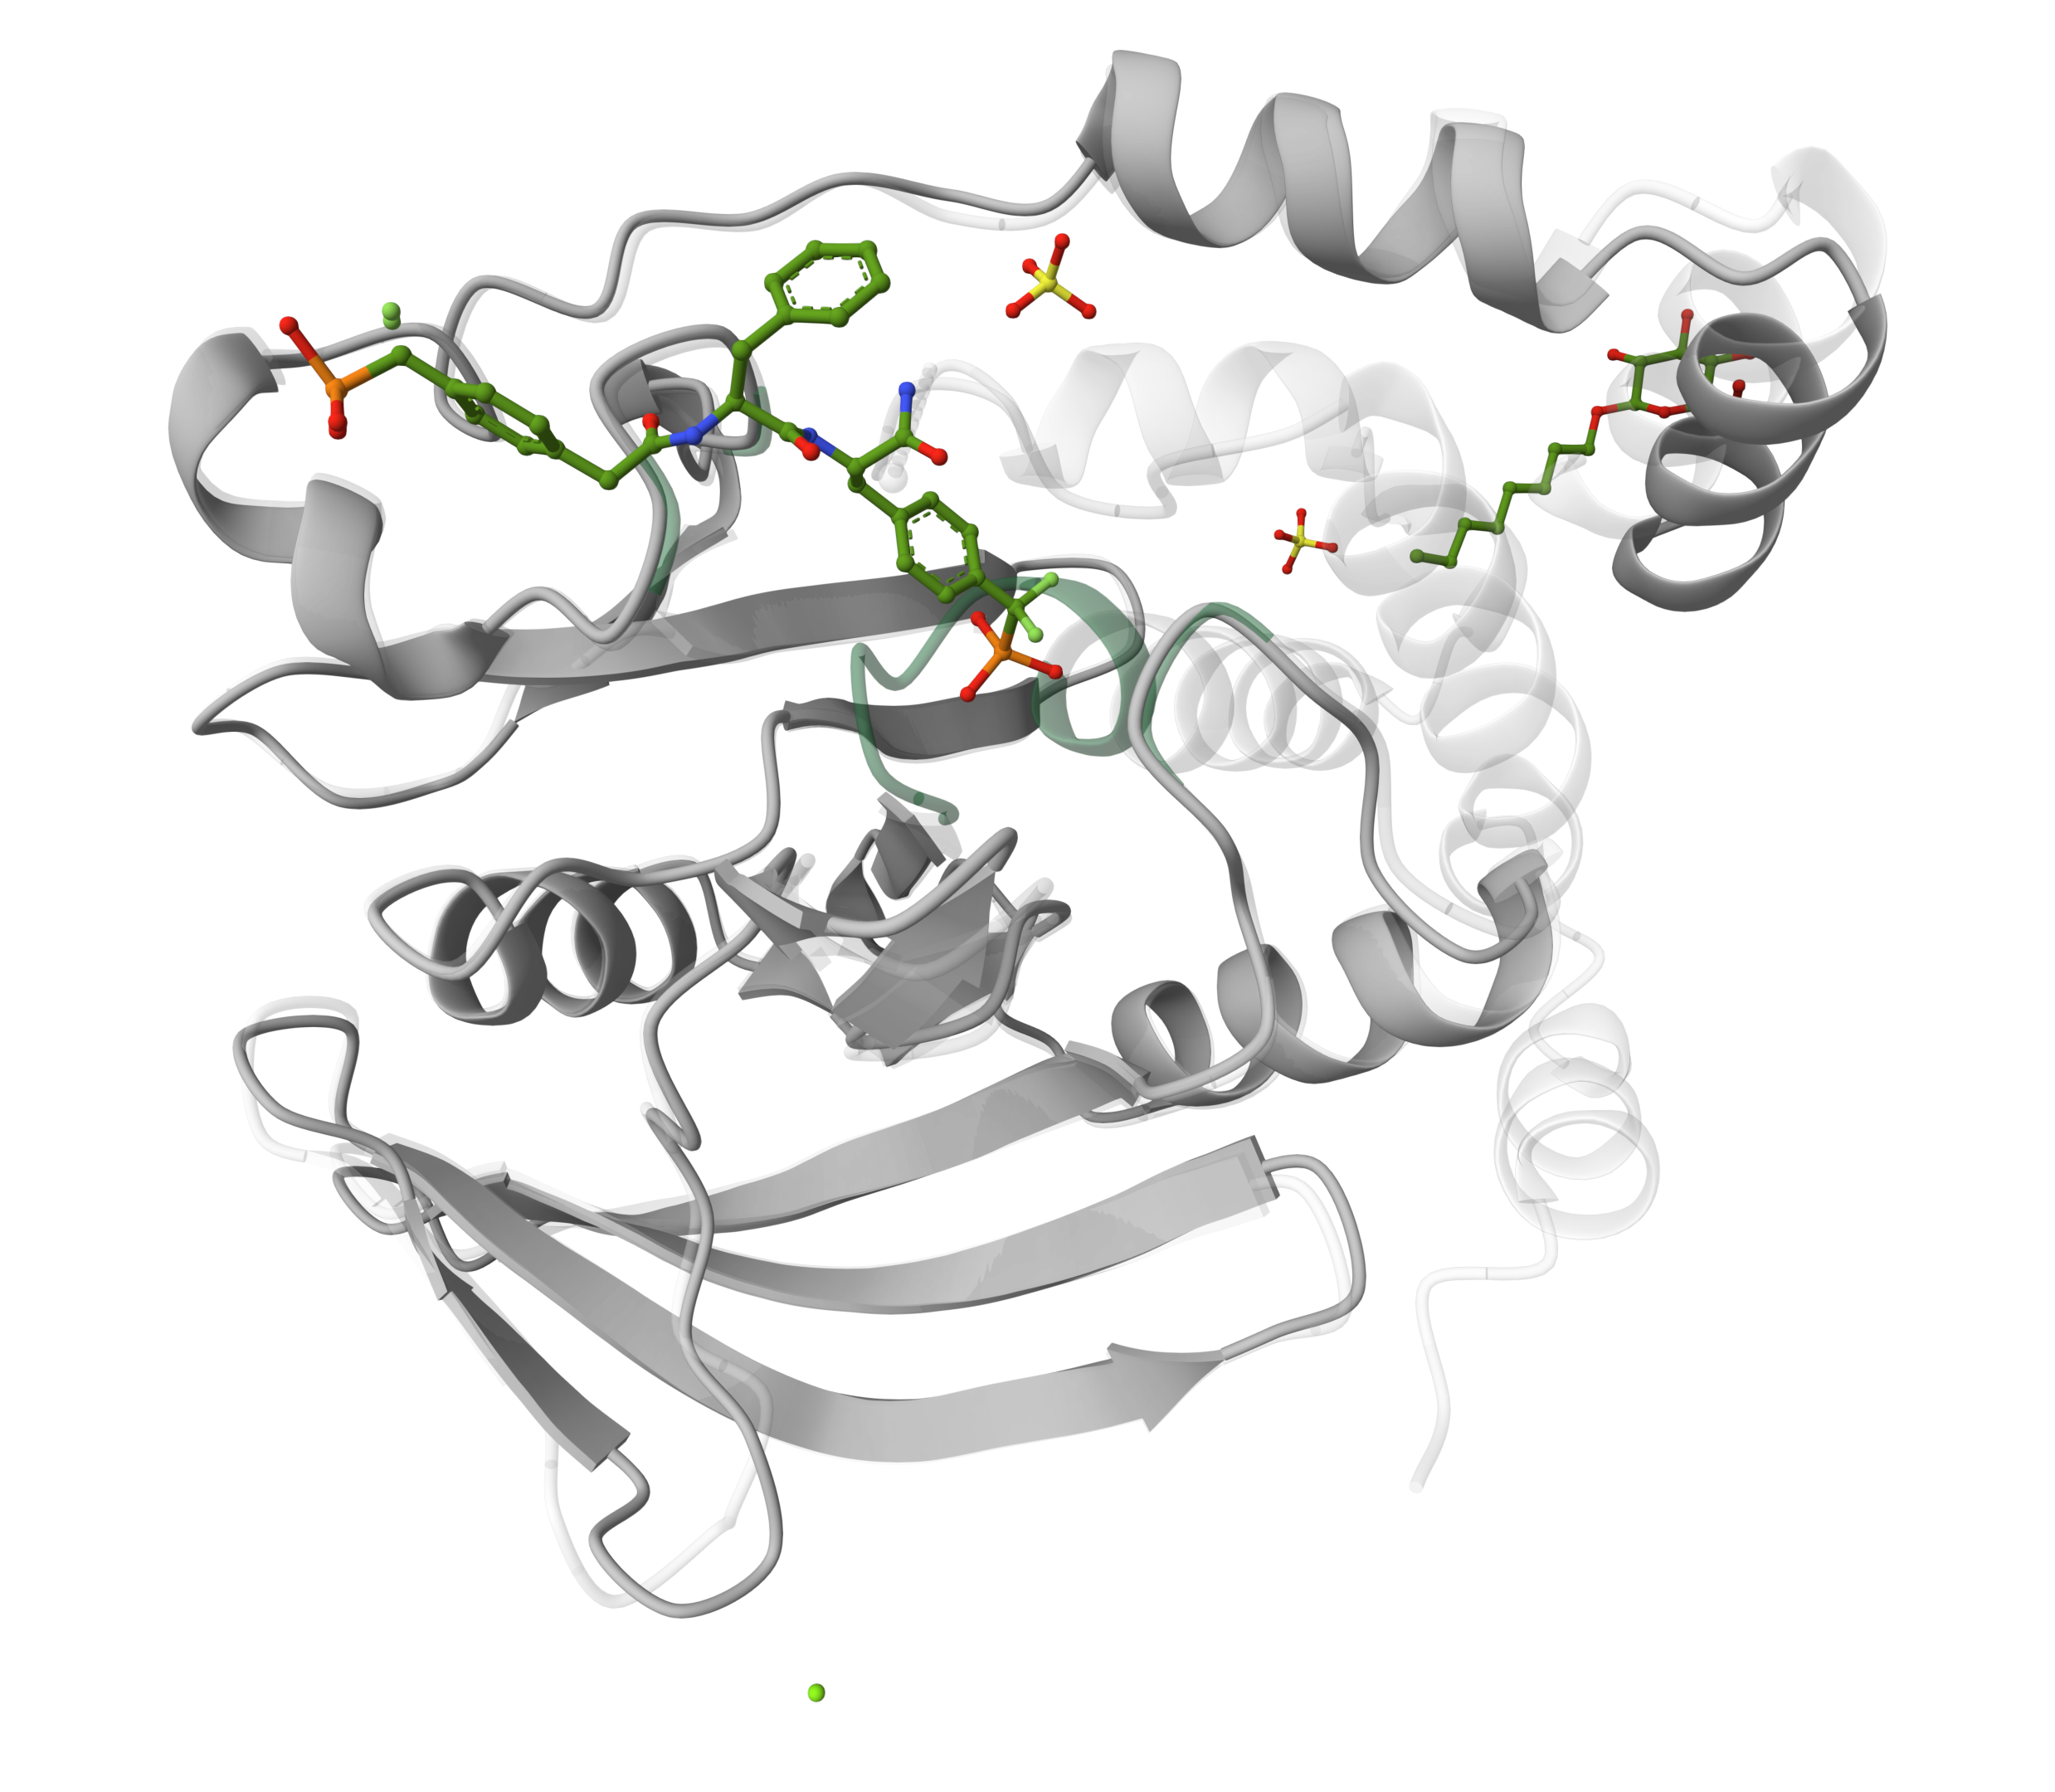
\includegraphics[width=\textwidth]{img/trajectory_animation.png}
    \caption{Example of trajectory animation demonstrating conformational changes between the input structure 1PTY (Crystal Structure of Protein Tyrosine Phosphatase 1B Complexed with Two Phosphotyrosine Molecules) and 2CNE (Structural Insights into the Design of Nonpeptidic Isothiazolidinone - Containing Inhibitors of Protein Tyrosine Phosphatase 1B). The input structure is displayed with 50\% transparency, while the target holo structure is rendered at full opacity. The ligand is represented in ball-and-stick format. Visualized using Mol* in CryptoShow.}
    \label{fig:trajectory-animation}
\end{figure}

Although this process generates a trajectory, it is important to note that this represents only a simple interpolation of residue coordinates. The trajectory does not depict actual conformational changes, but rather provides a smooth transition between the two structures. To capture genuine conformational dynamics, one would need to perform molecular dynamics simulations, which are computationally intensive and require significant time investment \cite{schlitter1993targeted}.

The source code for the trajectory animation functionality can be found in the \lstinline!backend/trajectory_generator! directory. As with the prediction and clustering components, the implementation details in the actual pipeline will be covered in Chapter \ref{chap:software}.


\section{Frontend}
\label{sec:frontend}

The frontend of the CryptoShow application is designed to provide an intuitive and user-friendly interface for the pipeline described in Chapter~\ref{chap:methodology}. The main technologies used for the frontend development include TypeScript, React, and Mol* (see Section~\ref{sec:molstar}), which is a powerful molecular visualization library. 

\subsection{NginX}
\label{sec:nginx}

The main component is NginX \cite{reese2008nginx}, which serves as a reverse proxy to many services and serves as one endpoint for the frontend. There are multiple configurations for NginX, which are defined in the \lstinline!frontend/nginx! files. We want to serve the frontend application in all cases, which is described by the default configuration. However, to improve user experience, we also provide configurations for TLS/SSL encryption, which is recommended for production environments. Moreover, we provide a configuration for the monitoring proxy endpoint, which is used to monitor the Celery tasks and queues (more details in Section~\ref{sec:tests-monitoring}). The NginX server listens on port 80 for HTTP requests and port 443 for HTTPS requests. The configuration files specify the root directory for static files, the location of the API endpoints, and the proxy settings for the backend service.

NginX does not support different behaviors for different environment variable values, so the final configuration file is generated on the fly using a simple Bash script. This script is executed during the Docker container startup, allowing for dynamic configuration based on the environment variables.

\subsection{React and TypeScript}
\label{sec:react-typescript}

The application is built using React\footnote{Available at \url{https://react.dev/}.}, a popular TypeScript library for creating web applications. This decision was made as React still remains state-of-the-art, and TypeScript provides strong typing and better developer experience compared to JavaScript. The frontend libraries are installed using the Bun\footnote{Available at \url{https://bun.sh/}.} package manager, which is known for its speed and efficiency (compared to Node.js). The source codes are transpiled and bundled using Vite\footnote{Available at \url{https://vitejs.dev/}.}, a modern build tool for TypeScript. The bundled files are then served by NginX, which is configured to serve static files from the \lstinline!frontend/dist! directory.

The component structure follows a modular approach, with each component defined in its own file and CSS style. The main entry point for the React application is the \lstinline!frontend/src/main.tsx! file, which renders the main \lstinline!App! component. The application is organized into several \lstinline|src| subdirectories:

\begin{itemize}
    \item \textbf{components} - Contains reusable components, such as tables, forms, and other UI elements.
    \item \textbf{pages} - Defines the page layouts, such as the home page, results page, about page, and error page.
    \item \textbf{hooks} - Includes custom React hooks for managing state and side effects.
    \item \textbf{contexts} - Provides React contexts for managing global state - variables that need to be accessed by multiple components.
    \item \textbf{providers} - Contains React providers for managing global state.
\end{itemize}

At the same level as the \lstinline|src| directory, there is a \lstinline!public! directory, which contains static files, such as images, icons, and HTML files. The \lstinline!index.html! file serves as the main entry point for the application, where the React application is mounted.

The React architecture follows the standard practices, beginning with \lstinline|HomePage|. This page serves as the landing page of the application, providing the user with an input table to enter the PDB ID or upload a custom protein structure. This logic is implemented in the aforementioned file and the \lstinline|InputTable| component. After computing the prediction, the user is presented with the \lstinline|Visualization| page. This page is split into several main components, such as the \lstinline|ResultTable|, \lstinline|MolstarControls| and Mol* visualization component (handled in the \lstinline|MolstarComponent| file), which is covered in Section~\ref{sec:molstar-frontend}.

Some of the component state is managed directly by the components themselves, while state that needs to be shared across multiple components is managed using React contexts. This approach allows better code organization and avoids prop drilling.

\xxx{TODO: add some code snippets}

\subsection{Mol*}
\label{sec:molstar-frontend}

Opposedly to other frontend components, the Mol* library requires a more detailed explanation, as it is a complex library with many features, but limited documentation. As described in Section~\ref{sec:molstar}, Mol* is a powerful molecular visualization library that provides advanced features for visualizing and interacting with molecular structures. It is used in the CryptoShow application to visualize the predicted cryptic binding sites and the trajectory animations.

Mol* does not work as a standard React component, but rather is rendered in a separate div element within the React component tree. This requires a different approach to the state management. The div element is defined in the \lstinline|Visualization| component, and the Mol* viewer is initialized in the \lstinline|MolstarComponent| component via the \lstinline|initializePlugin| method.

Once the viewer has been initialized, the structure data is loaded into the viewer. At this stage, several protein representations are created, allowing users to switch between them via dedicated methods. The loading functionality is implemented in the \lstinline|loadStructure| method. Optionally, a trajectory file can also be loaded alongside the structure to enable the trajectory animation described in Section~\ref{sec:trajectory}.

After the structure is loaded into the viewer, the visualization of the predicted binding sites can be performed. For each pocket found in the JSON object returned by the backend (see Section~\ref{sec:prediction-backend}), new, colored representations are generated for the corresponding predicted cryptic binding sites. This approach allows users to easily distinguish the CBSs and select their preferred representation type alongside the main structure.

The file also provides additional methods essential for the visualization process, including adjusting structure transparency, retrieving residue selections, obtaining detailed residue information with coordinates, and overpainting the structure.

For the trajectory animation, the original structure is displayed with an opacity of 0.5, making it visually distinct from the apo-holo pair returned by AHoJ. The aligned structure and the generated trajectory file from the backend are both loaded into the Mol* viewer. The trajectory file contains the intermediate states of the aligned structure. Mol* then animates these states, visually illustrating the conformational transition of the protein.

\xxx{TODO: screenshots - maybe refer to the 4th chapter instead}

\section{Tests and Monitoring}
\label{sec:tests-monitoring}

To improve the reliability and stability of the CryptoShow application, multiple monitoring and testing tools have been set up. These tools help to ensure that the application is running, and that the Celery tasks are executed correctly. The monitoring tools also provide insights into the performance of the application and the Celery workers.

First of all, basic health checks are implemented in the Docker Compose file. Docker periodically checks the health of the services and restarts them if they are not healthy. The health checks are defined in the \lstinline!docker-compose.yml! file, where each service has a \lstinline|healthcheck| section that specifies the command to run to check the health of the service. For example, the backend service checks if the FastAPI server is running by sending a request to the \lstinline!/health! endpoint. These health checks are being run in every case, regardless of the environment variable values. If a Docker healthcheck fails, Docker marks the container as unhealthy. This information can be used to restart the container.

To enhance the monitoring capabilities, Flower is used to monitor the Celery tasks and queues. Flower provides a web-based interface that allows users to view the status of the Celery workers, the tasks in the queue, and the task execution times. It is configured to run on port 5555 and can be accessed via the \lstinline!/flower! endpoint thanks to NginX. The Flower service communicates with the Redis service to retrieve task information.

Moreover, Grafana, Prometheus and Celery Exporter work together to provide a comprehensive monitoring solution with a user-friendly dashboard. Prometheus serves as a data source for Grafana, receiving metrics from the Celery workers via the Celery Exporter. The Celery Exporter is a lightweight service that exposes Celery metrics to Prometheus, allowing it to scrape and store these metrics. Grafana then visualizes the metrics in a dashboard. The Grafana service is configured to run on port 3001 and can be accessed via the \lstinline!/grafana! endpoint. Prometheus itself is configured to run on port 9090 and can be accessed via the \lstinline!/prometheus! endpoint. The configuration files for Prometheus and Grafana are located in the \lstinline!monitoring! directory. Figure~\ref{fig:grafana} shows an example of the Grafana dashboard.

\begin{figure}[htpb]
    \centering
    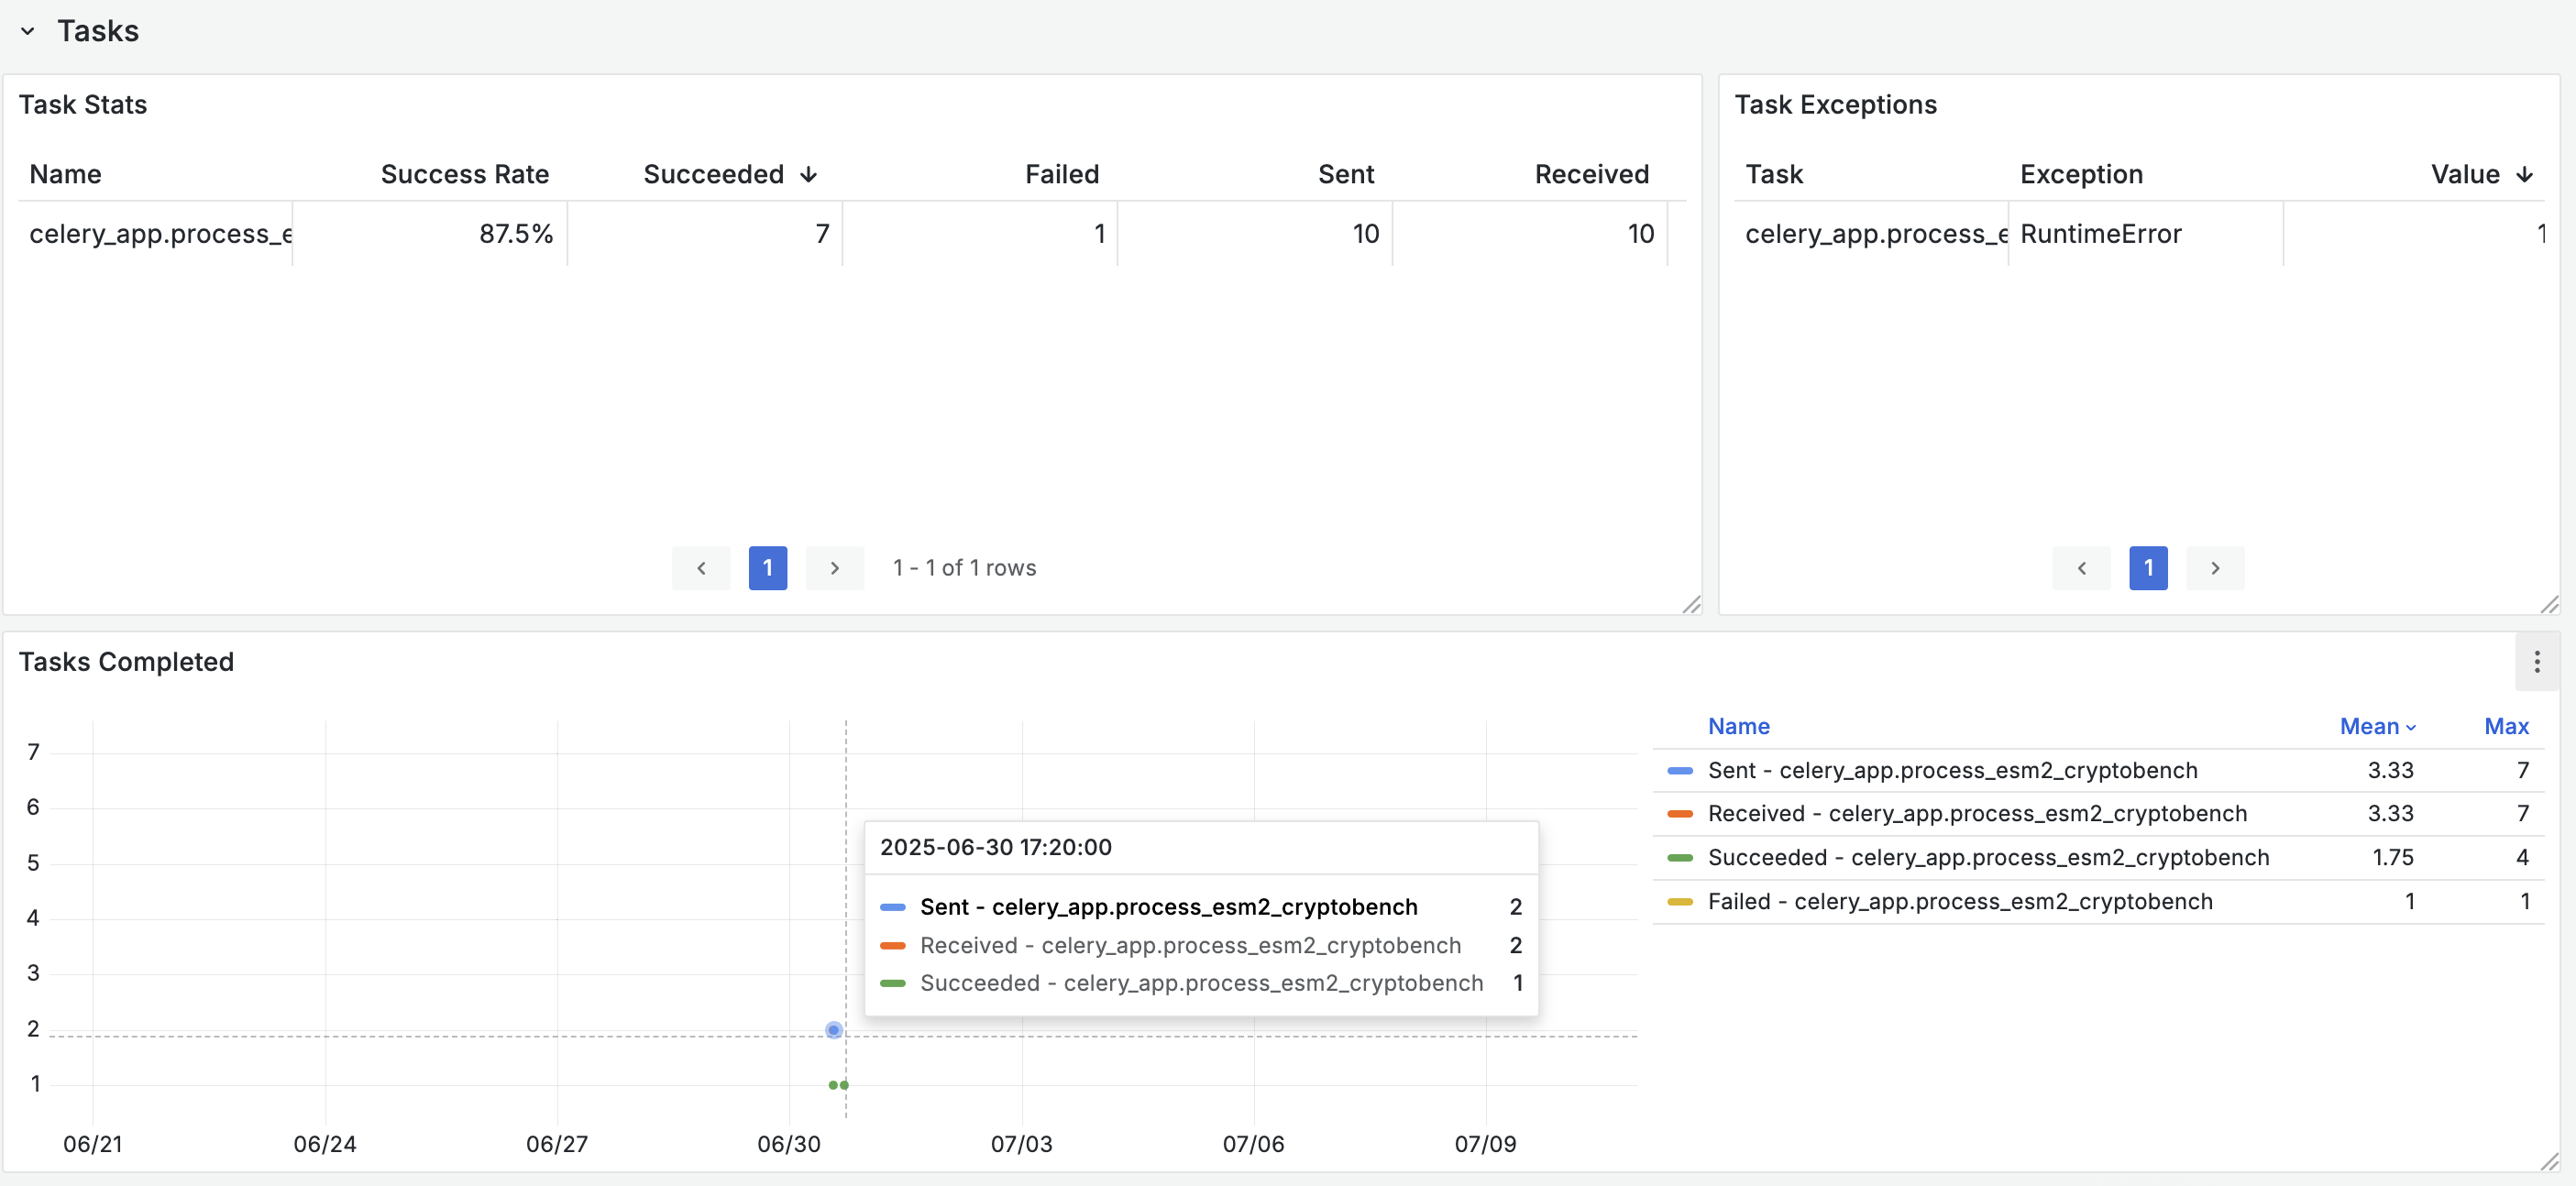
\includegraphics[width=\textwidth]{img/grafana.png}
    \caption{Screenshot of the Grafana dashboard displaying Prometheus statistics.}
    \label{fig:grafana}
\end{figure}

Although the monitoring services are useful, they are not always necessary for the application to function. This is the reason why a monitoring flag mechanism has been introduced. The \lstinline!monitoring-flag! service creates a flag file that enables the monitoring services, while the \lstinline!remove-monitoring-flag! service removes the flag file, disabling the monitoring services. The container to remove the flag file is run every time the application is started, so the monitoring services are disabled by default. If the developer wants to enable the monitoring services, they do so by running the Docker Compose command with the \lstinline|--profile monitoring| option, which turns on the monitoring profile. This activates the \lstinline!monitoring-flag! service, creating the flag file and enabling the monitoring services. The monitoring services are then accessible via the respective endpoints thanks to the flexible configuration of NginX. Otherwise, the endpoints are not available, and the containers are not started to save RAM and CPU resources.

As most of the functionality of the frontend is visual, the frontend is tested manually. Still, some bugs can be caught using Sentry\footnote{Available at \url{https://sentry.io/}}, which is a tool for error tracking and monitoring. Sentry is configured to capture errors in the frontend, providing detailed information about the errors, including stack traces. This allows quicker identification of the bugs in the application. The Sentry service is integrated using the environment variables in the \lstinline|frontend| directory (see the example environment file \lstinline!frontend/.env.template!).

\section{Deployment}
\label{sec:deployment}

CryptoShow is distributed as a fully dockerized application, enabling simple deployment and scalability. It can be deployed on any server with Docker Compose support, requiring at least 32 GB of RAM and 8 CPU cores.

Before starting, the \lstinline|.env| file must be created in the root folder to specify required environment variables. The variables are listed in the \lstinline|.env.template| file, and include the following:

\begin{itemize}
    \item \textbf{ENABLE\_SSL}: \texttt{<true|false>} - Enable or disable SSL. Recommended for production.
    \item \textbf{SSL\_PATH}: \texttt{<path to ssl certificate and key folder>} - Path to SSL certificate and key (not required if SSL is disabled).
    \item \textbf{DOMAIN}: \texttt{<domain name>} - Domain name for the deployment.
    \item \textbf{UID}: \texttt{<user id (default: 2727)>} - Linux user ID for running containers. Make sure that the user has sufficient permissions to the filesystem.
    \item \textbf{GID}: \texttt{<group id (default: 2727)>} - Linux group ID for running containers.
    \item \textbf{HTPASSWD\_PATH}: \texttt{<path to htpasswd file>} - Path to HTTP basic auth password file for monitoring access.
    \item \textbf{HTTP\_PROXY}: \texttt{<http proxy URL>} - HTTP proxy URL for development behind a proxy (optional).
    \item \textbf{HTTPS\_PROXY}: \texttt{<https proxy URL>} - HTTPS proxy URL (optional).
\end{itemize}

Once the \lstinline|.env| file has been created, the next step is to build the Docker images for all services specified in the \lstinline!docker-compose.yml! file. This can be accomplished using the standard \lstinline|docker compose build| command. Alternatively, Docker Bake\footnote{Available at \url{https://docs.docker.com/build/bake/}.}, a tool that enables parallel building of multiple Docker images, may be used. To use Docker Bake, run \lstinline|docker buildx bake|.

CryptoShow supports accelerated computations using the CUDA architecture. To specify whether the application should utilize GPU or CPU resources, the developer must select the appropriate mode by passing the \lstinline|--profile <cpu/gpu>| flag when building and running the application with Docker Compose.

As described in Section~\ref{sec:tests-monitoring}, monitoring features can be enabled by including the monitoring profile when running Docker Compose: \lstinline|--profile monitoring|.

Before deploying the application, make sure to enable incoming and outcoming traffic to ports 80 and 443 (if using SSL). Also, note that multiple ports are exposed:

\begin{itemize}
    \item \textbf{80/tcp} - HTTP (frontend, NginX)
    \item \textbf{443/tcp} - HTTPS (frontend, NginX)
    \item \textbf{3001/tcp} - Grafana (monitoring dashboard, optional)
    \item \textbf{5000/tcp} - Backend API (FastAPI)
    \item \textbf{5555/tcp} - Flower (Celery monitoring, optional)
    \item \textbf{6379/tcp} - Redis (message broker)
    \item \textbf{9090/tcp} - Prometheus (monitoring, optional)
    \item \textbf{9808/tcp} - Celery Exporter (monitoring, optional)
\end{itemize}

Blocking direct access to the other ports is not strictly required, but leaving the ports open can lead into unauthorized access to the monitoring.

Once the infrastructure is built, the application can be started using the \lstinline|docker compose up| command, along with any relevant profile flags as described above. The application will then be accessible on port 80 or 443, depending on the value of the ENABLE\_SSL environment variable.

Detailed step-by-step instructions, including SSL certificate generation and file permission configuration, are provided in the \lstinline|README| file.

\subsection{Local Frontend Development}
\label{sec:local-frontend-development}

For faster development, the frontend application can be run locally. First, install the required dependencies using the Bun package manager with \lstinline|bun i|. Then, start the development server using \lstinline|bun run dev|. The frontend will be accessible at port 3000.

\subsection{Local Backend Development}
\label{sec:local-backend-development}

While running the backend services locally is technically possible, it requires installing multiple tools and frameworks, making the process complicated. Therefore, it is strongly recommended to use Docker for backend development. Developers may choose to modify the Dockerfile and Docker Compose configurations to enable hot reloading if desired, but this is not provided by default. For local development of the services, consult the relevant Dockerfiles and the Docker Compose file.

\chapter{User Documentation}
\label{chap:user-documentation}

This chapter provides user documentation for the CryptoShow application, including a brief introduction on how to use the application.

\section{How to Use}
\label{sec:how-to-use}

To use the CryptoShow application, either deploy it locally (see Section~\ref{sec:deployment}) or access the live version at \url{https://cryptoshow.cz}.

Upon opening the main page, an input table is displayed. Provide either a structure identifier (PDB or AlphaFold ID) or upload a PDB/mmCIF file. Once a valid structure is provided, the application will begin processing and displays the computation status. Processing time varies based on the structure size and server load.

Once the computation is finished, the user is presented with a link to the calculation results. After clicking the link, the user is redirected to the visualization page. The following elements are shown:

\begin{itemize}
    \item An interactive 3D visualization of the structure, allowing users to rotate and zoom. Residues that are part of detected cryptic binding sites are highlighted using distinct colors.
    \item A toolbox providing options to adjust visualization styles.
    \item A table listing the identified cryptic binding sites with expandable rows. Each entry includes details about the involved residues, their scores, and a PyMOL selection string for visualizing the site in PyMOL. For each pocket (in PDB structures), users can initiate an AHoJ query to obtain apo-holo pairs and visualize possible conformational changes. Results can also be downloaded as a ZIP archive.
\end{itemize}

The 3D visualization in Mol* with the toolbox is shown in Figure~\ref{fig:ui-molstar}. The results table with expandable rows is shown in Figure~\ref{fig:ui-table}.

\begin{figure}[htbp]
    \centering
    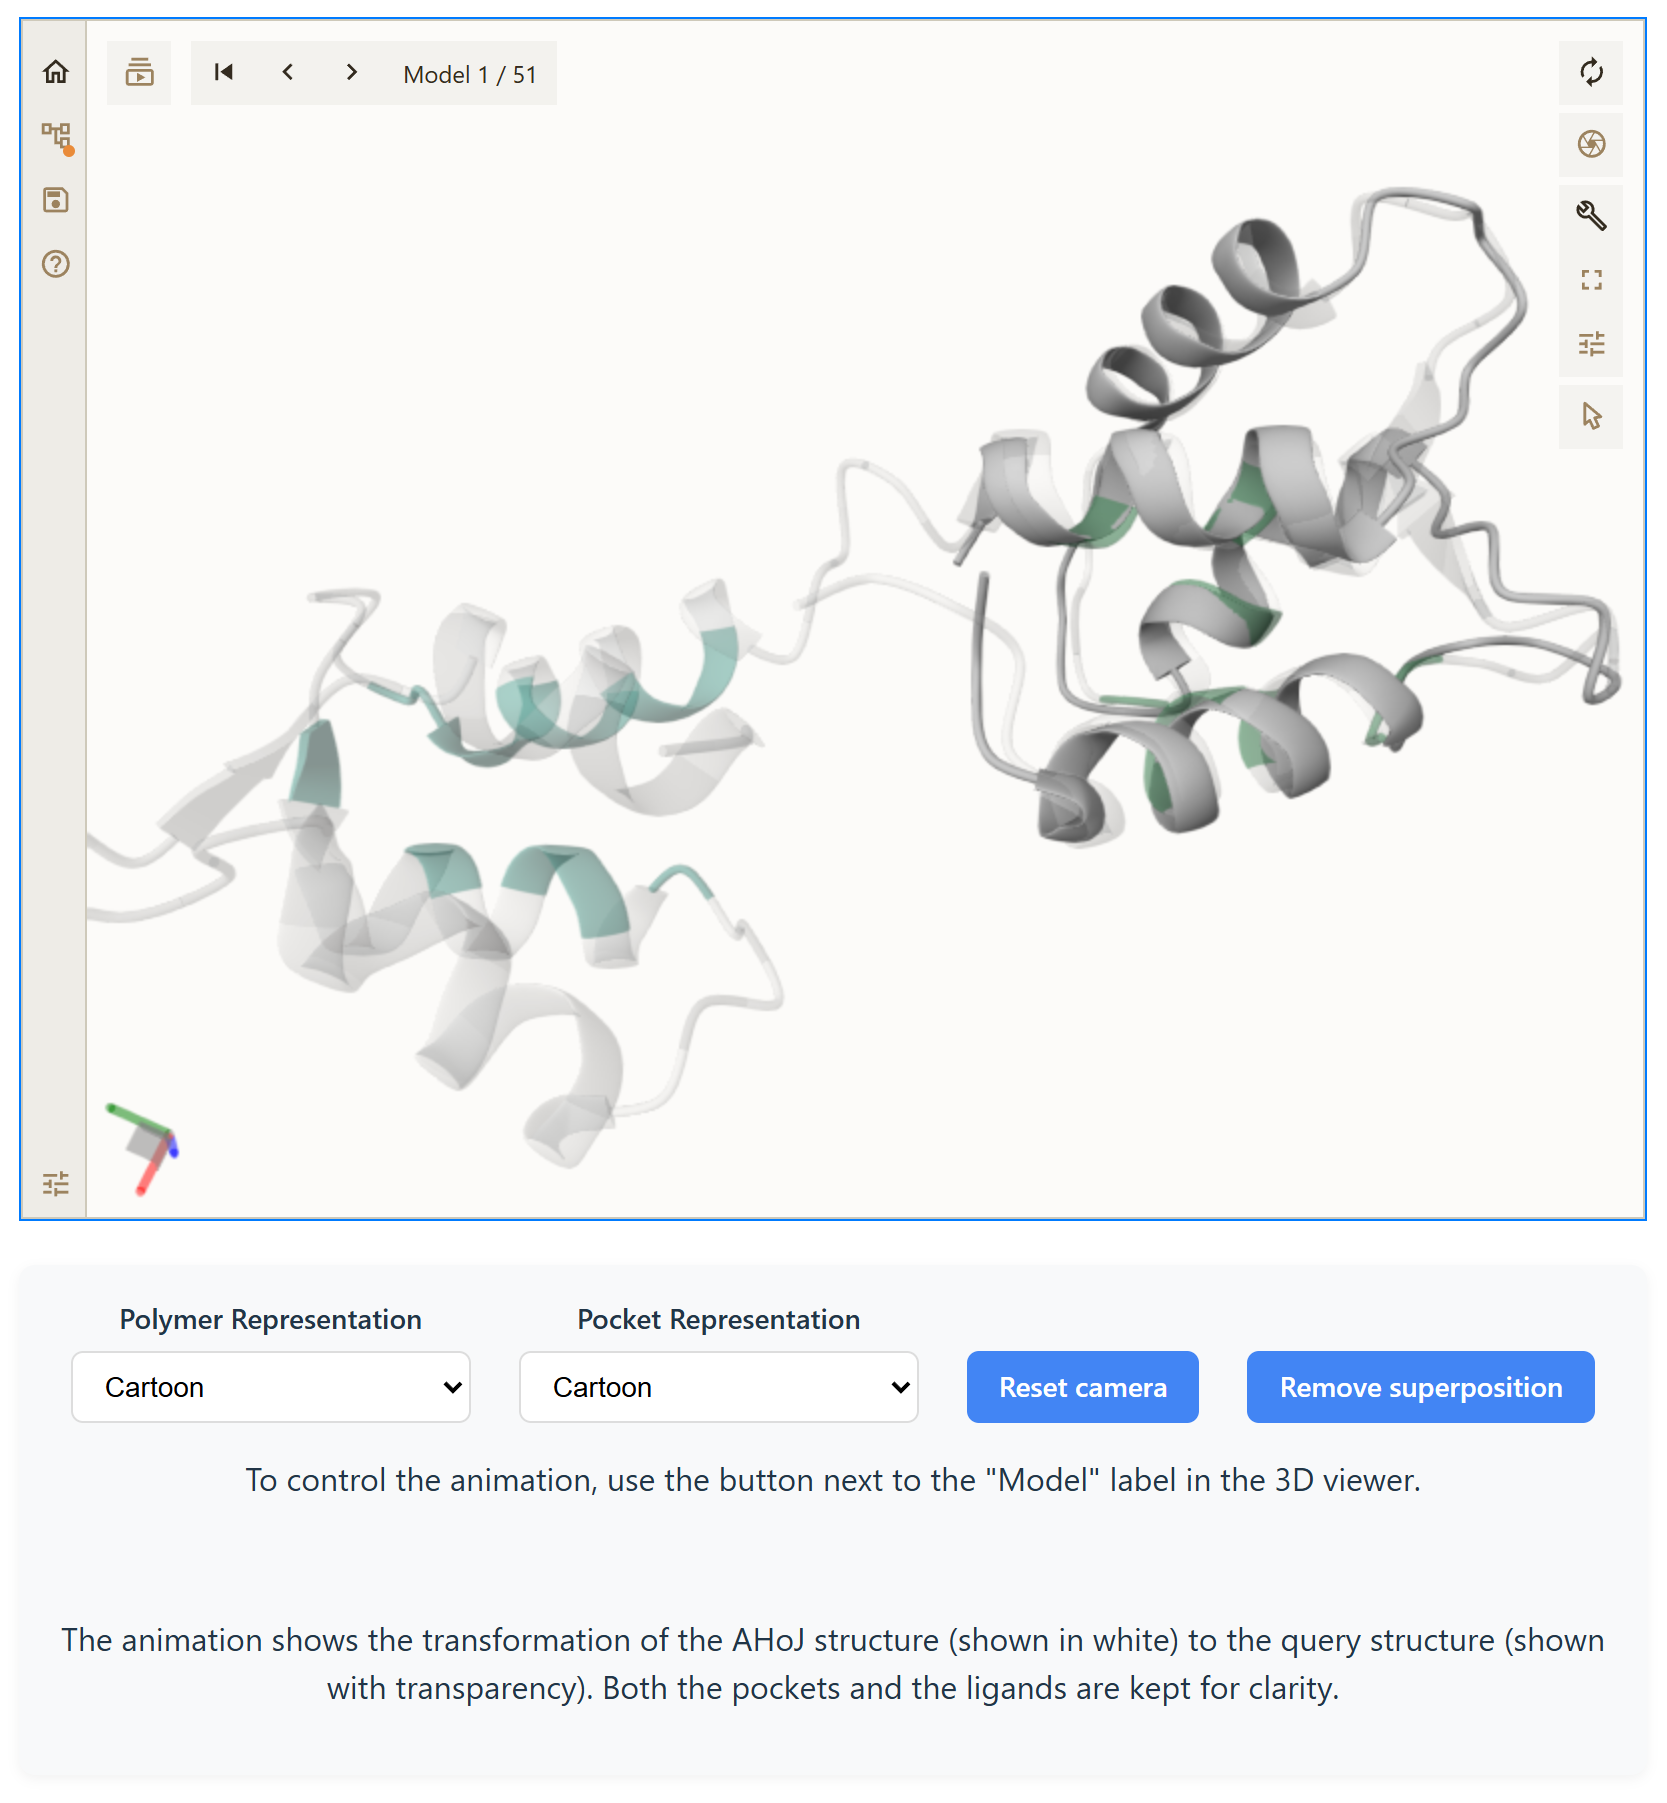
\includegraphics[width=\textwidth]{img/ui-molstar.png}
    \caption{Mol* 3D visualization of the protein structure of Calcium-free Calmodulin (1CFD), along with the Crystal Structure of Myosin-1c tail in complex with Calmodulin (4R8G), with the visualization toolbox underneath.}
    \label{fig:ui-molstar}
\end{figure}

\begin{figure}[htbp]
    \centering
    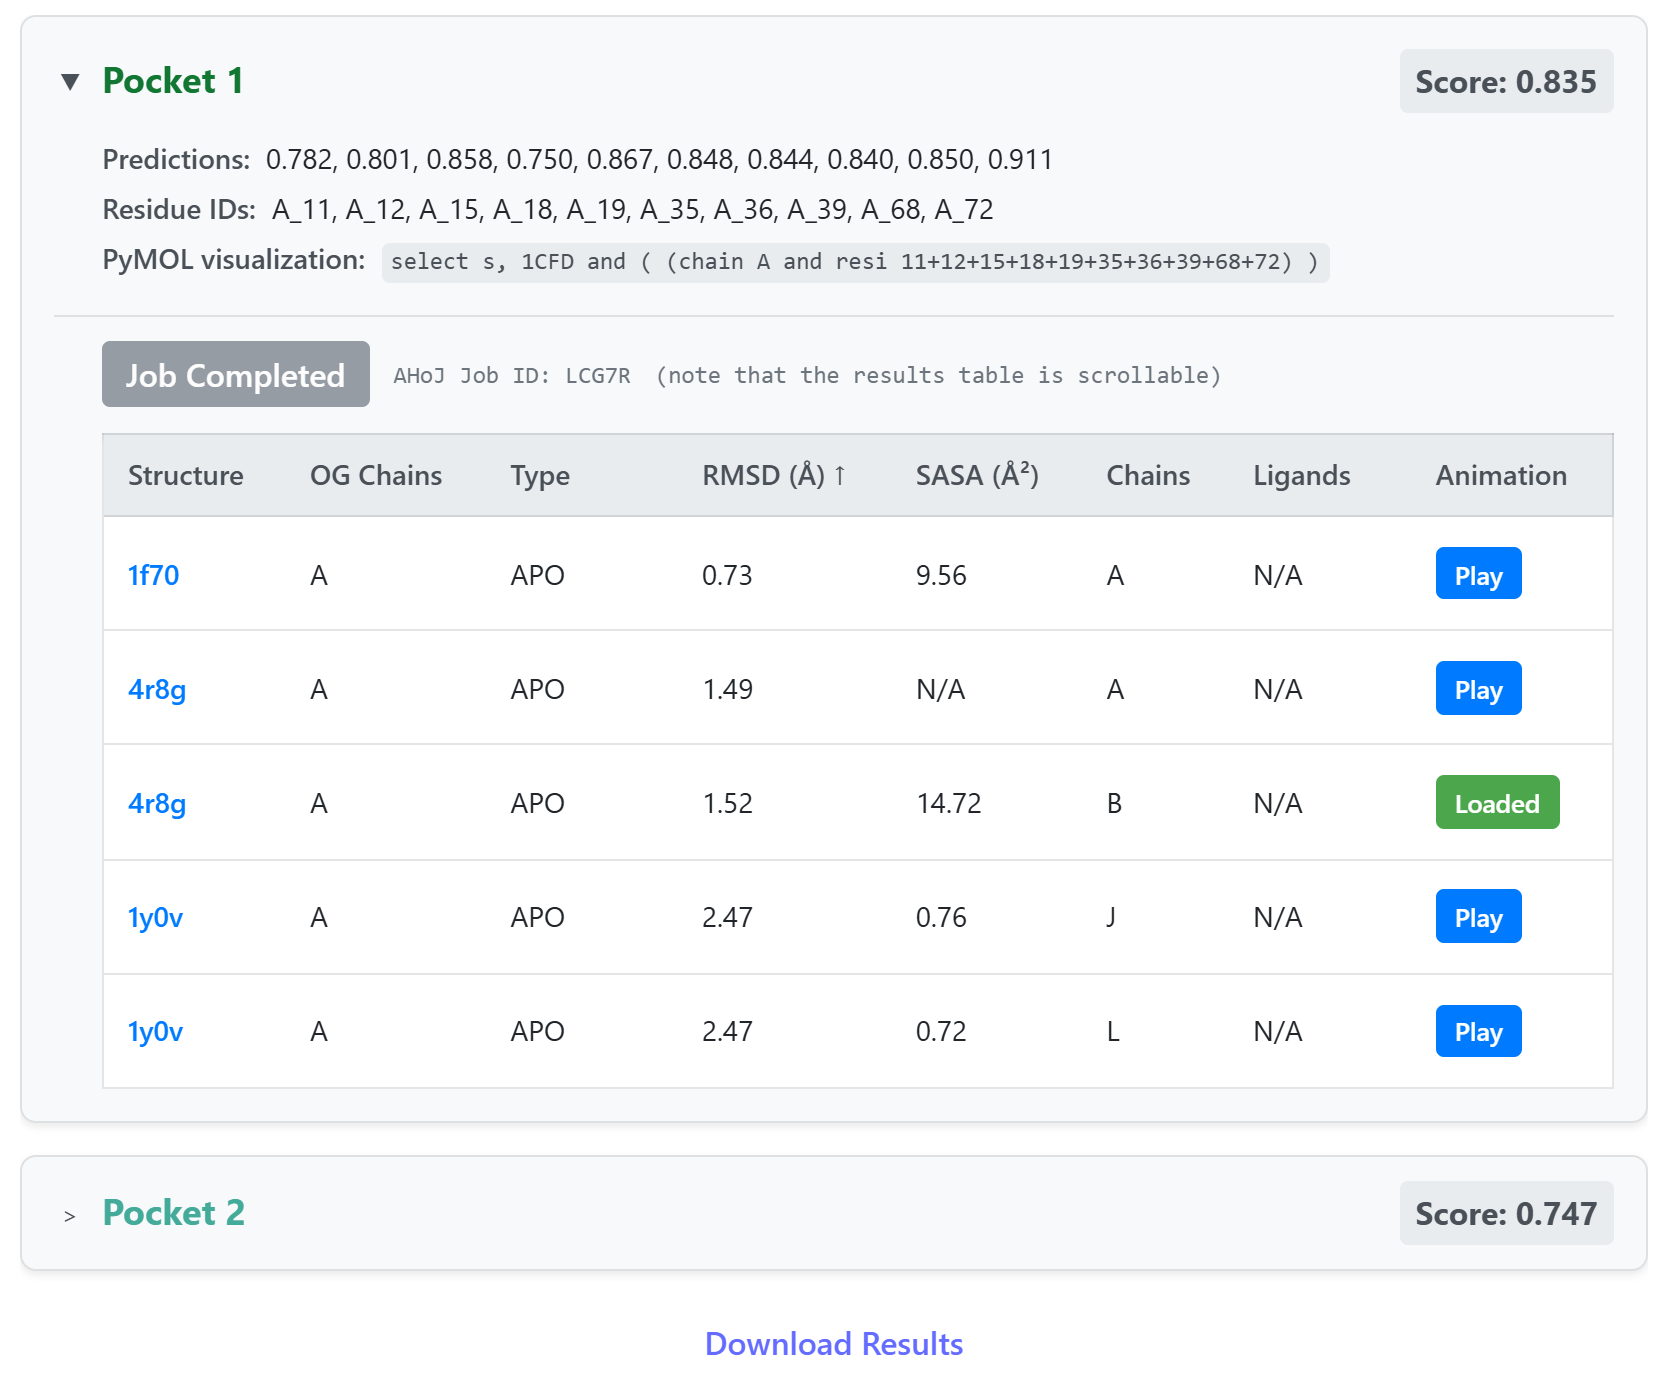
\includegraphics[width=\textwidth]{img/ui-table.png}
    \caption{Table of cryptic binding sites for the Calcium-free Calmodulin (1CFD) protein structure with expandable rows, showing details about the involved residues, their scores, and a PyMOL selection string for visualizing the site in PyMOL.}
    \label{fig:ui-table}
\end{figure}

\section{Use Case: Predicting Cryptic Binding Sites in DHFR}
\label{sec:use-case}

To illustrate the intended use of the CryptoShow application, we examine a real-world example from computational drug discovery. This scenario demonstrates how structural analysis and simulation tools can uncover cryptic binding sites in proteins—sites that are not evident in ligand-free structures but emerge in ligand-bound forms or during dynamic conformational changes. This example is inspired by the work of \citet{meller2023predicting}.

\subsection{Case Study: Dihydrofolate Reductase (DHFR)}
\label{subsec:dhfr-example}

As a case study, we use the protein dihydrofolate reductase (DHFR) from \textit{Escherichia coli}, an important target in antimicrobial drug development \cite{heaslet2009structural}. We begin with the apo structure, PDB ID \textbf{2W9T}, which shows DHFR in its unbound state with no visible deep binding pockets beyond the known active site.

Using the CryptoShow application, we predict potential cryptic pockets based solely on the apo structure. One binding site is identified near the so-called Met20 loop\footnote{The Met20 loop is a flexible segment of DHFR, named after the methionine amino acid at position 20 (residue ID 42 in this structure), and is known for its role in modulating access to the active site through conformational changes.}, a flexible region of the protein known to undergo conformational changes. Figure~\ref{fig:ui-cryptic-pocket} illustrates this prediction, with the Met20 loop highlighted in light yellow.

\begin{figure}[htbp]
    \centering
    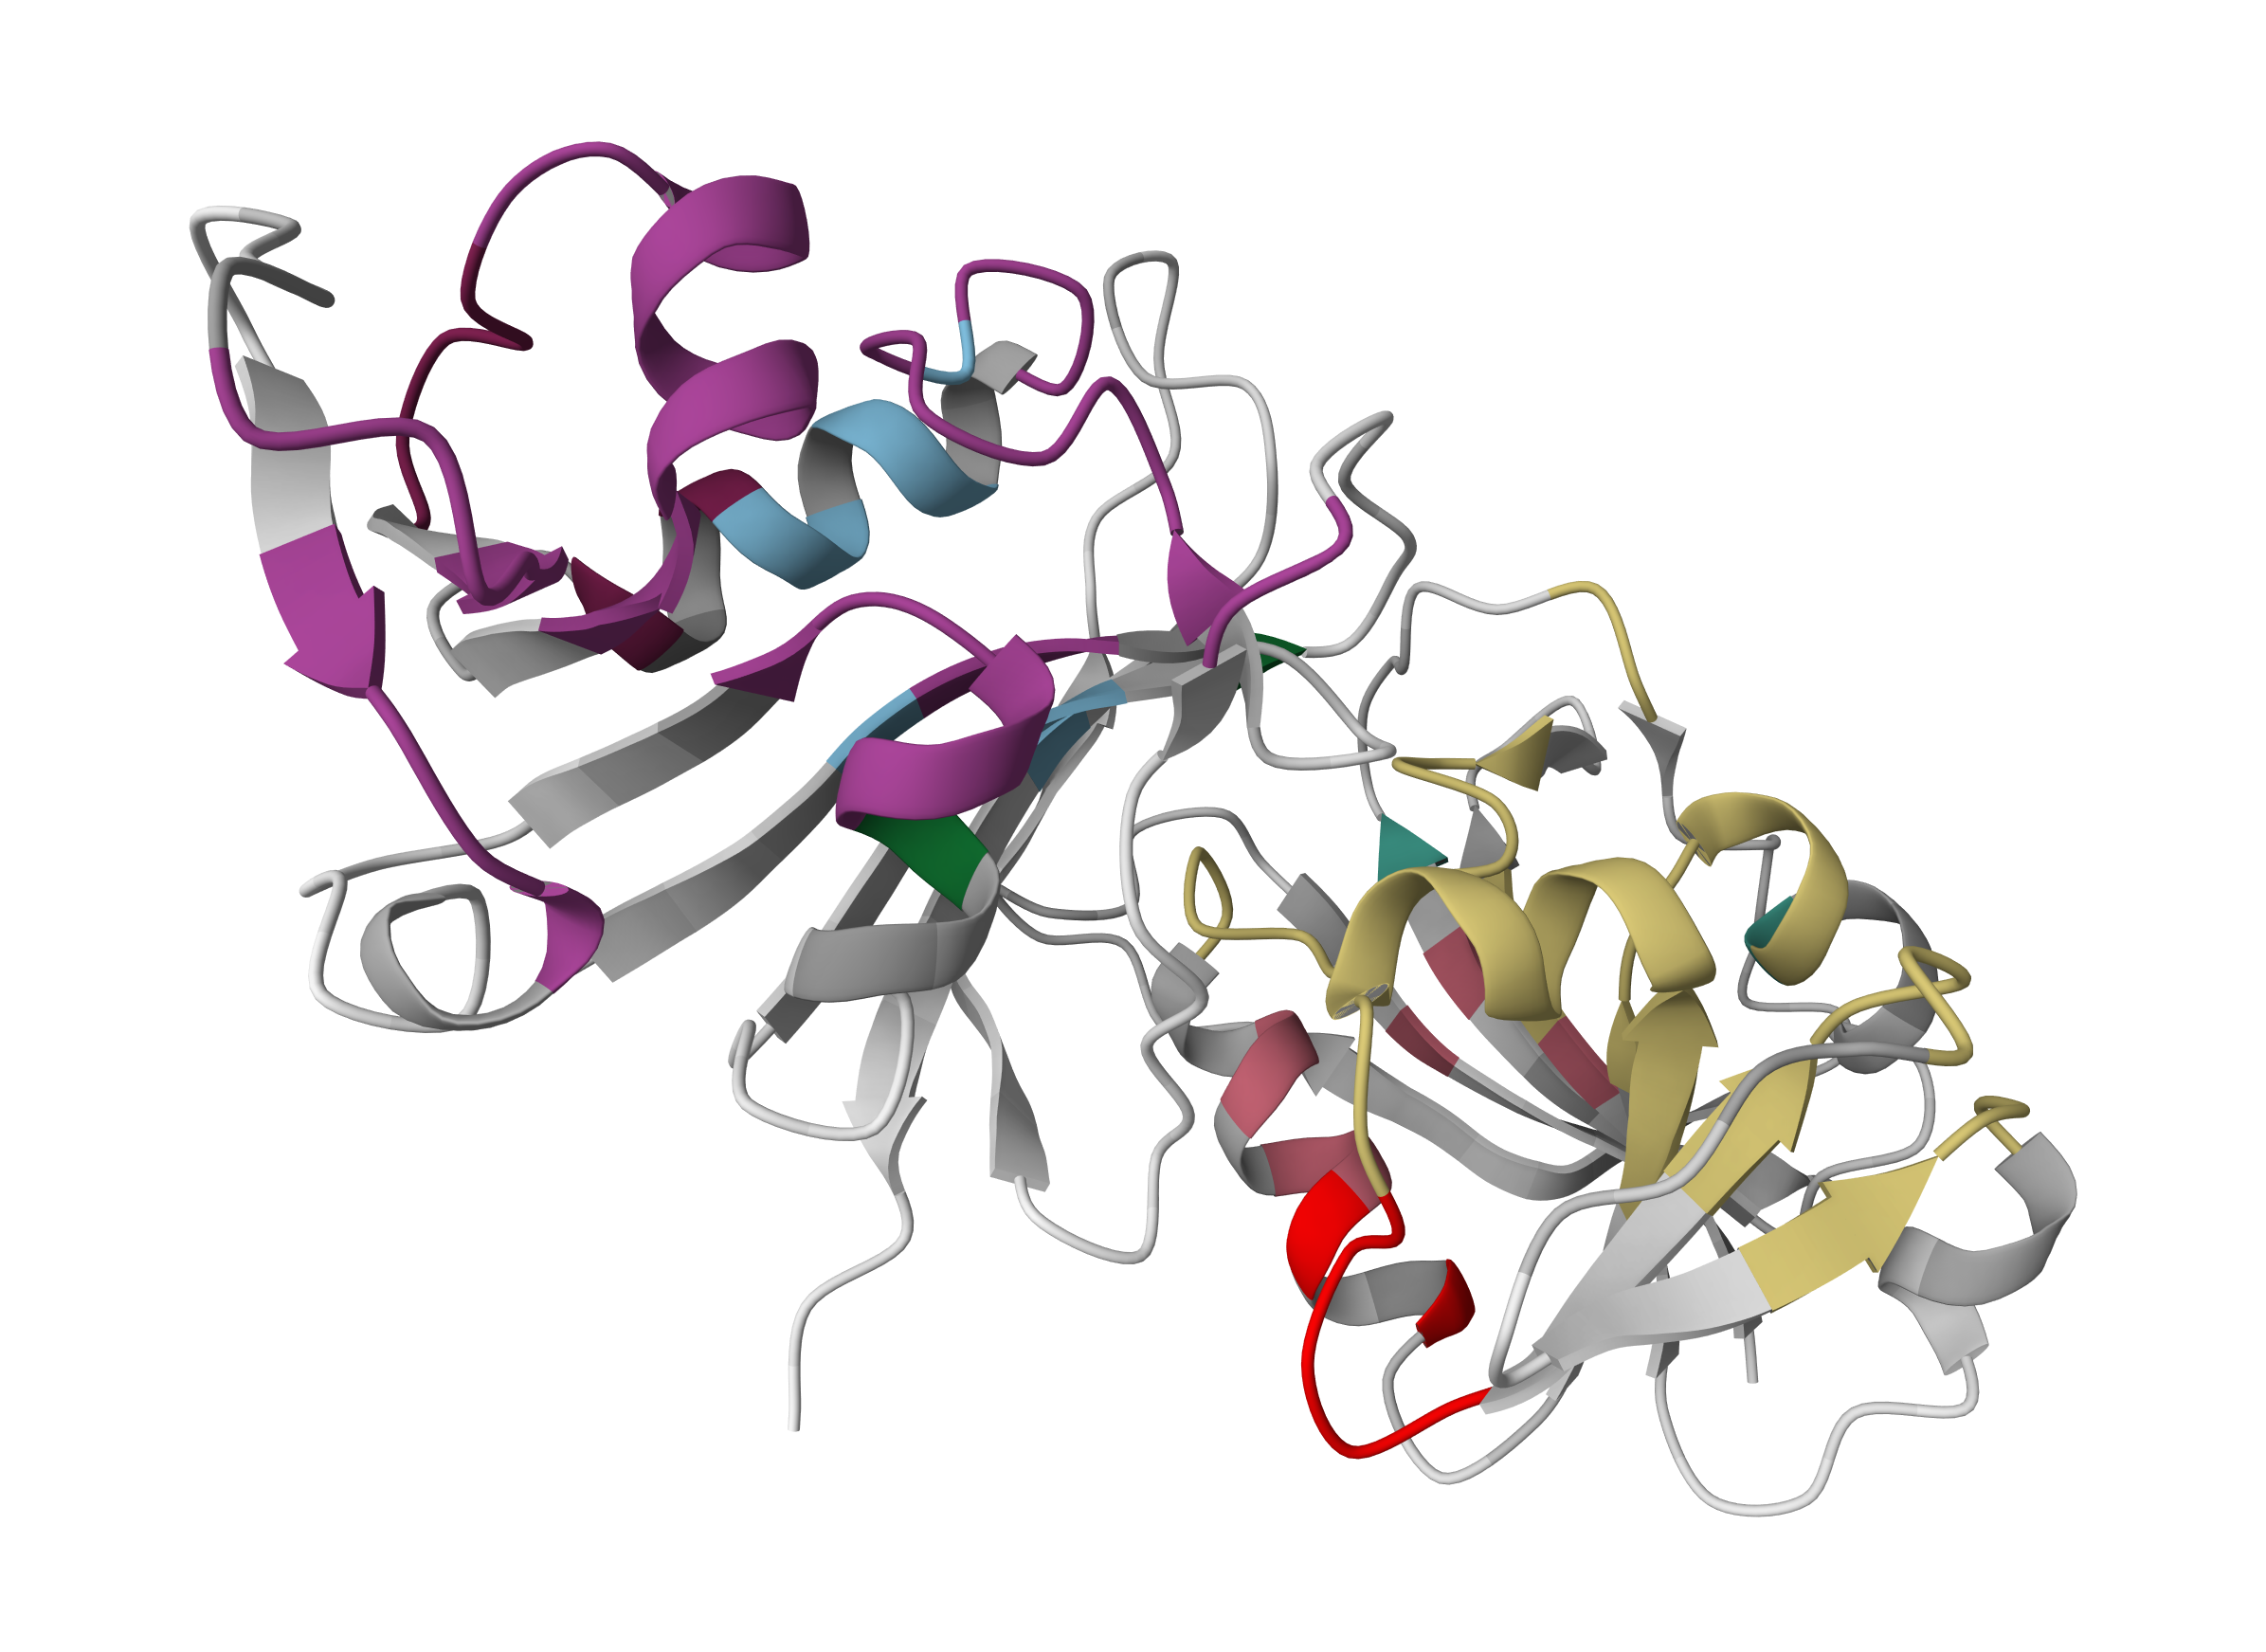
\includegraphics[width=\textwidth]{img/2w9t_prediction.png}
    \caption{Predicted cryptic binding sites in the apo structure of DHFR (PDB ID 2W9T) using the CryptoShow application. The pockets are highlighted in different colors, with the Met20 binding site shown in light yellow. Visualized using Mol*.}
    \label{fig:ui-cryptic-pocket}
\end{figure}

\subsection{Validation Using Holo Structure}
\label{subsec:holo-validation}

To evaluate the accuracy of the prediction, we consult the AHoJ database by clicking the button in the pocket details window (see Figure~\ref{fig:ahoj-btn}) to identify known holo structures of DHFR. Indeed, a holo form is available: PDB ID \textbf{2W9S}, in which the protein is bound to the antimicrobial drug Trimethoprim. In this structure, the Met20 loop shifts position, exposing a pocket that matches the one predicted by the CryptoShow application from the apo form. The conformational change of the Met20 loop can be visualized in the application. Figure~\ref{fig:2w9t_2w9s} presents this structural comparison.

\begin{figure}[htpb]
    \centering
    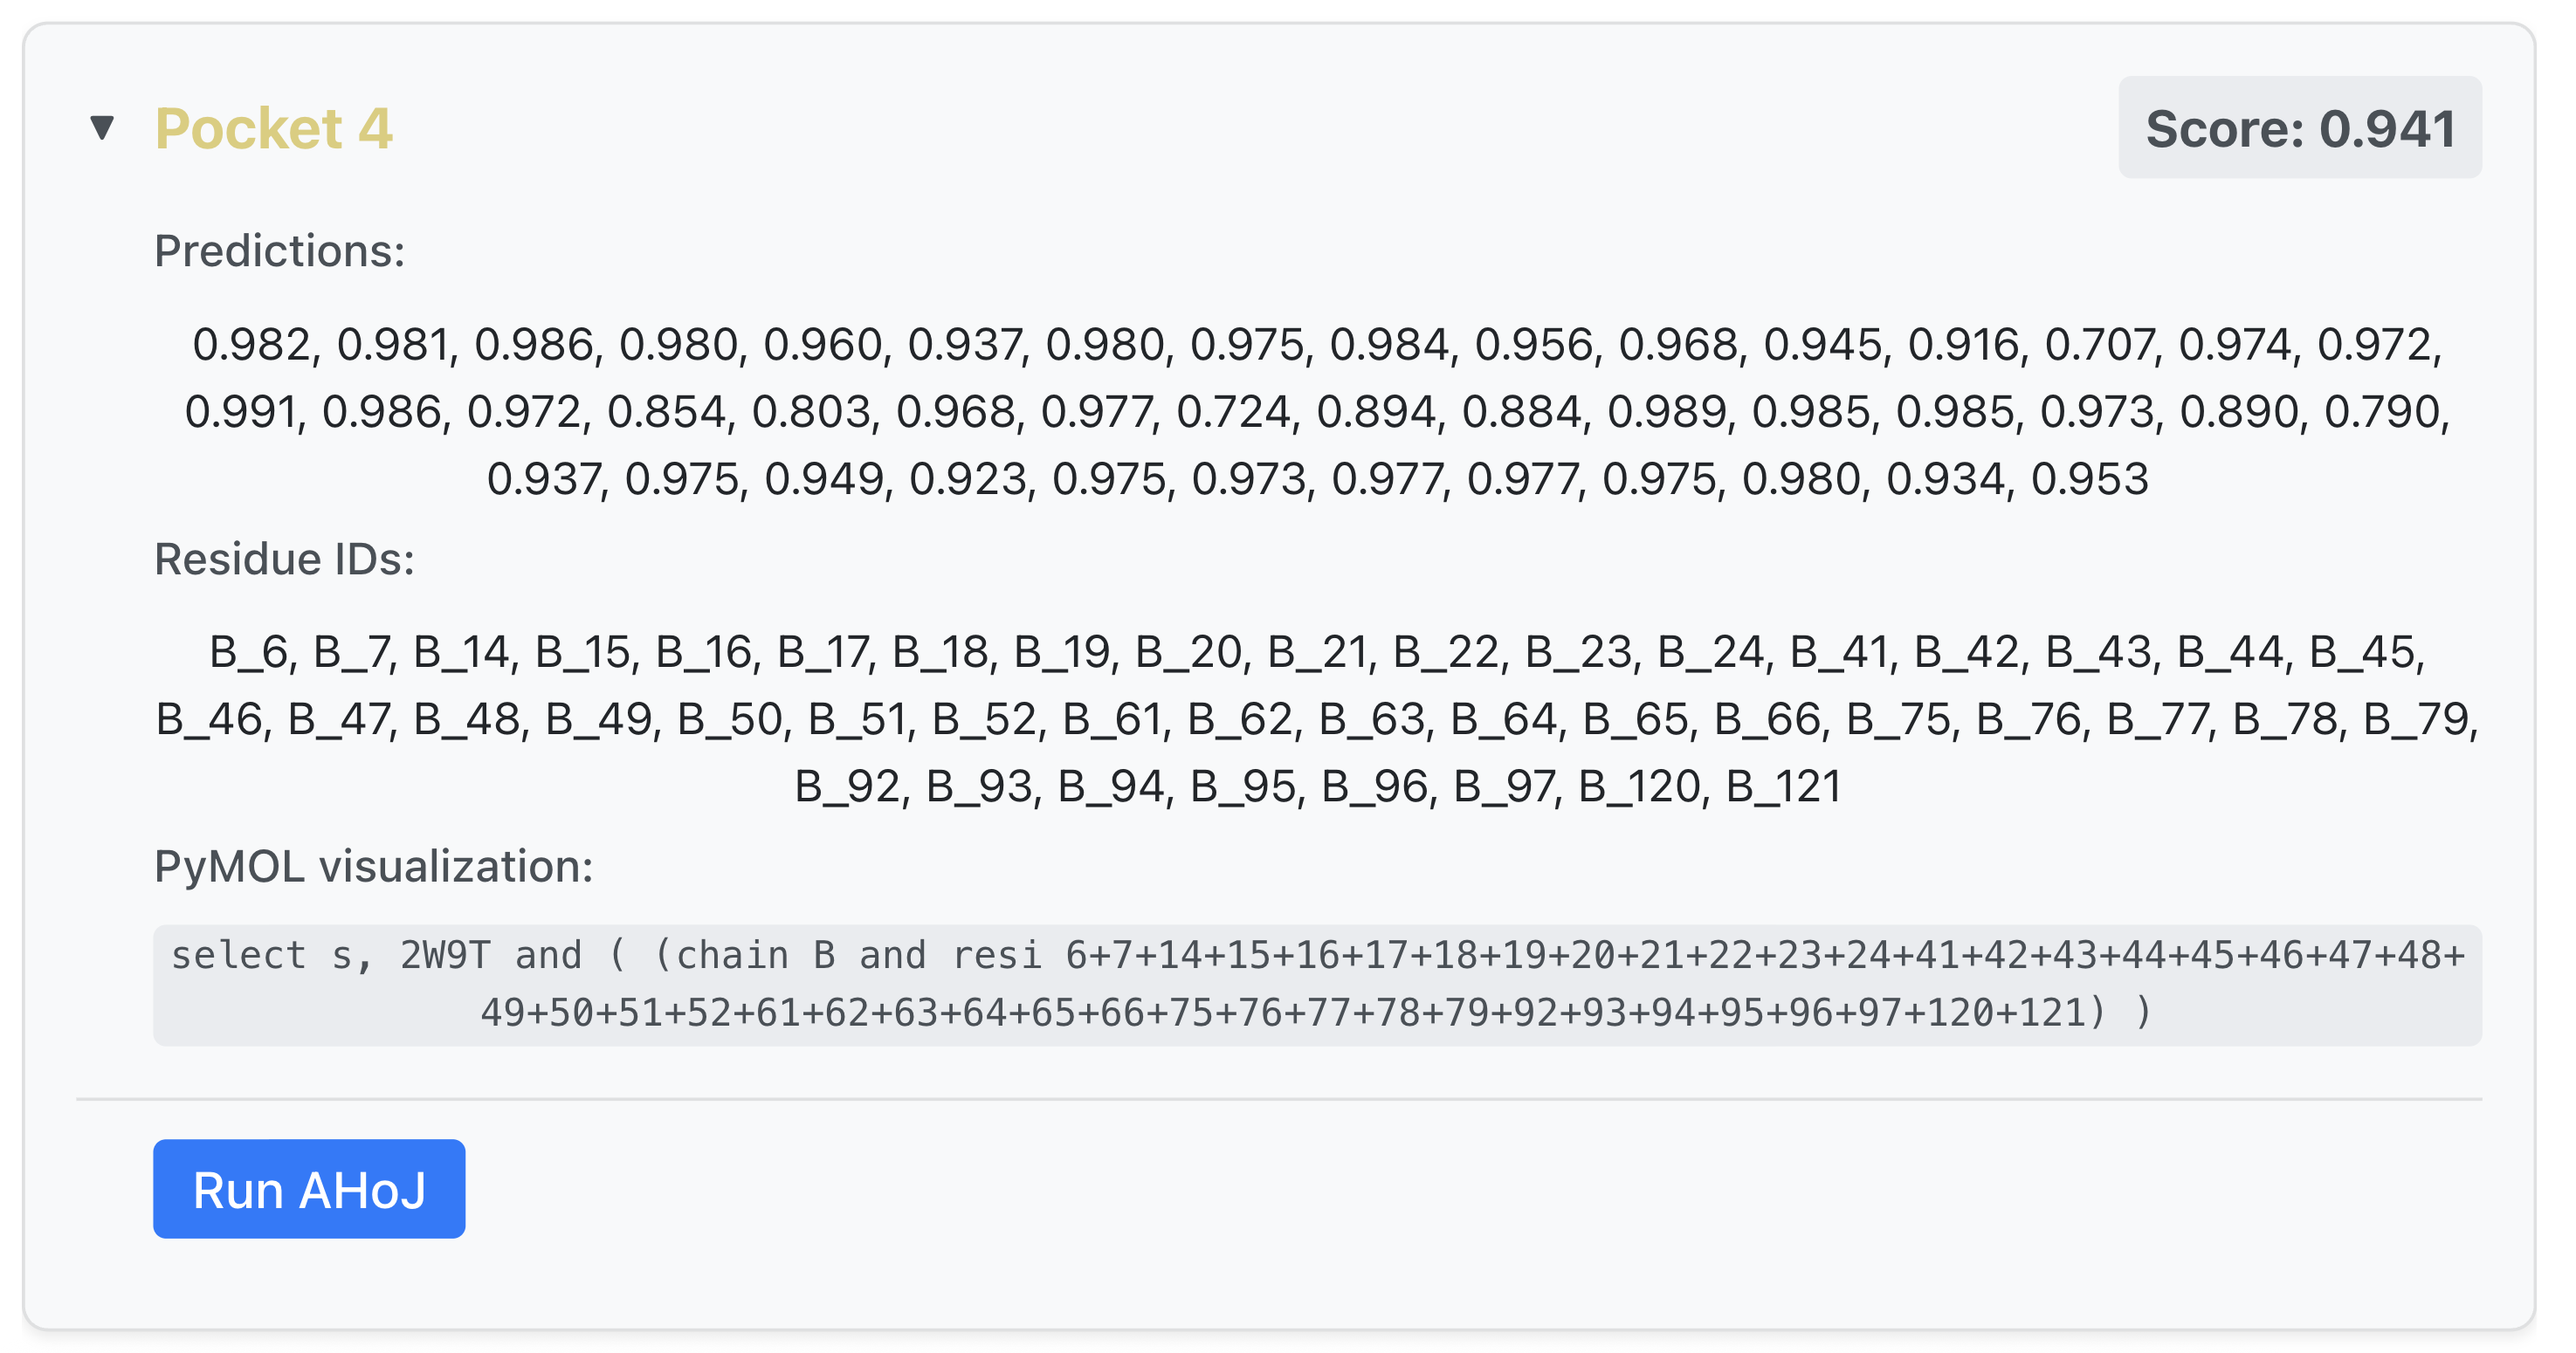
\includegraphics[width=\textwidth]{img/ahoj-btn.png}
    \caption{Details window for the Met20 loop CBS in the 2W9T protein structure. The AHoJ query can be initiated by clicking the button.}
    \label{fig:ahoj-btn}
\end{figure}

\begin{figure}[htpb]
    \centering
    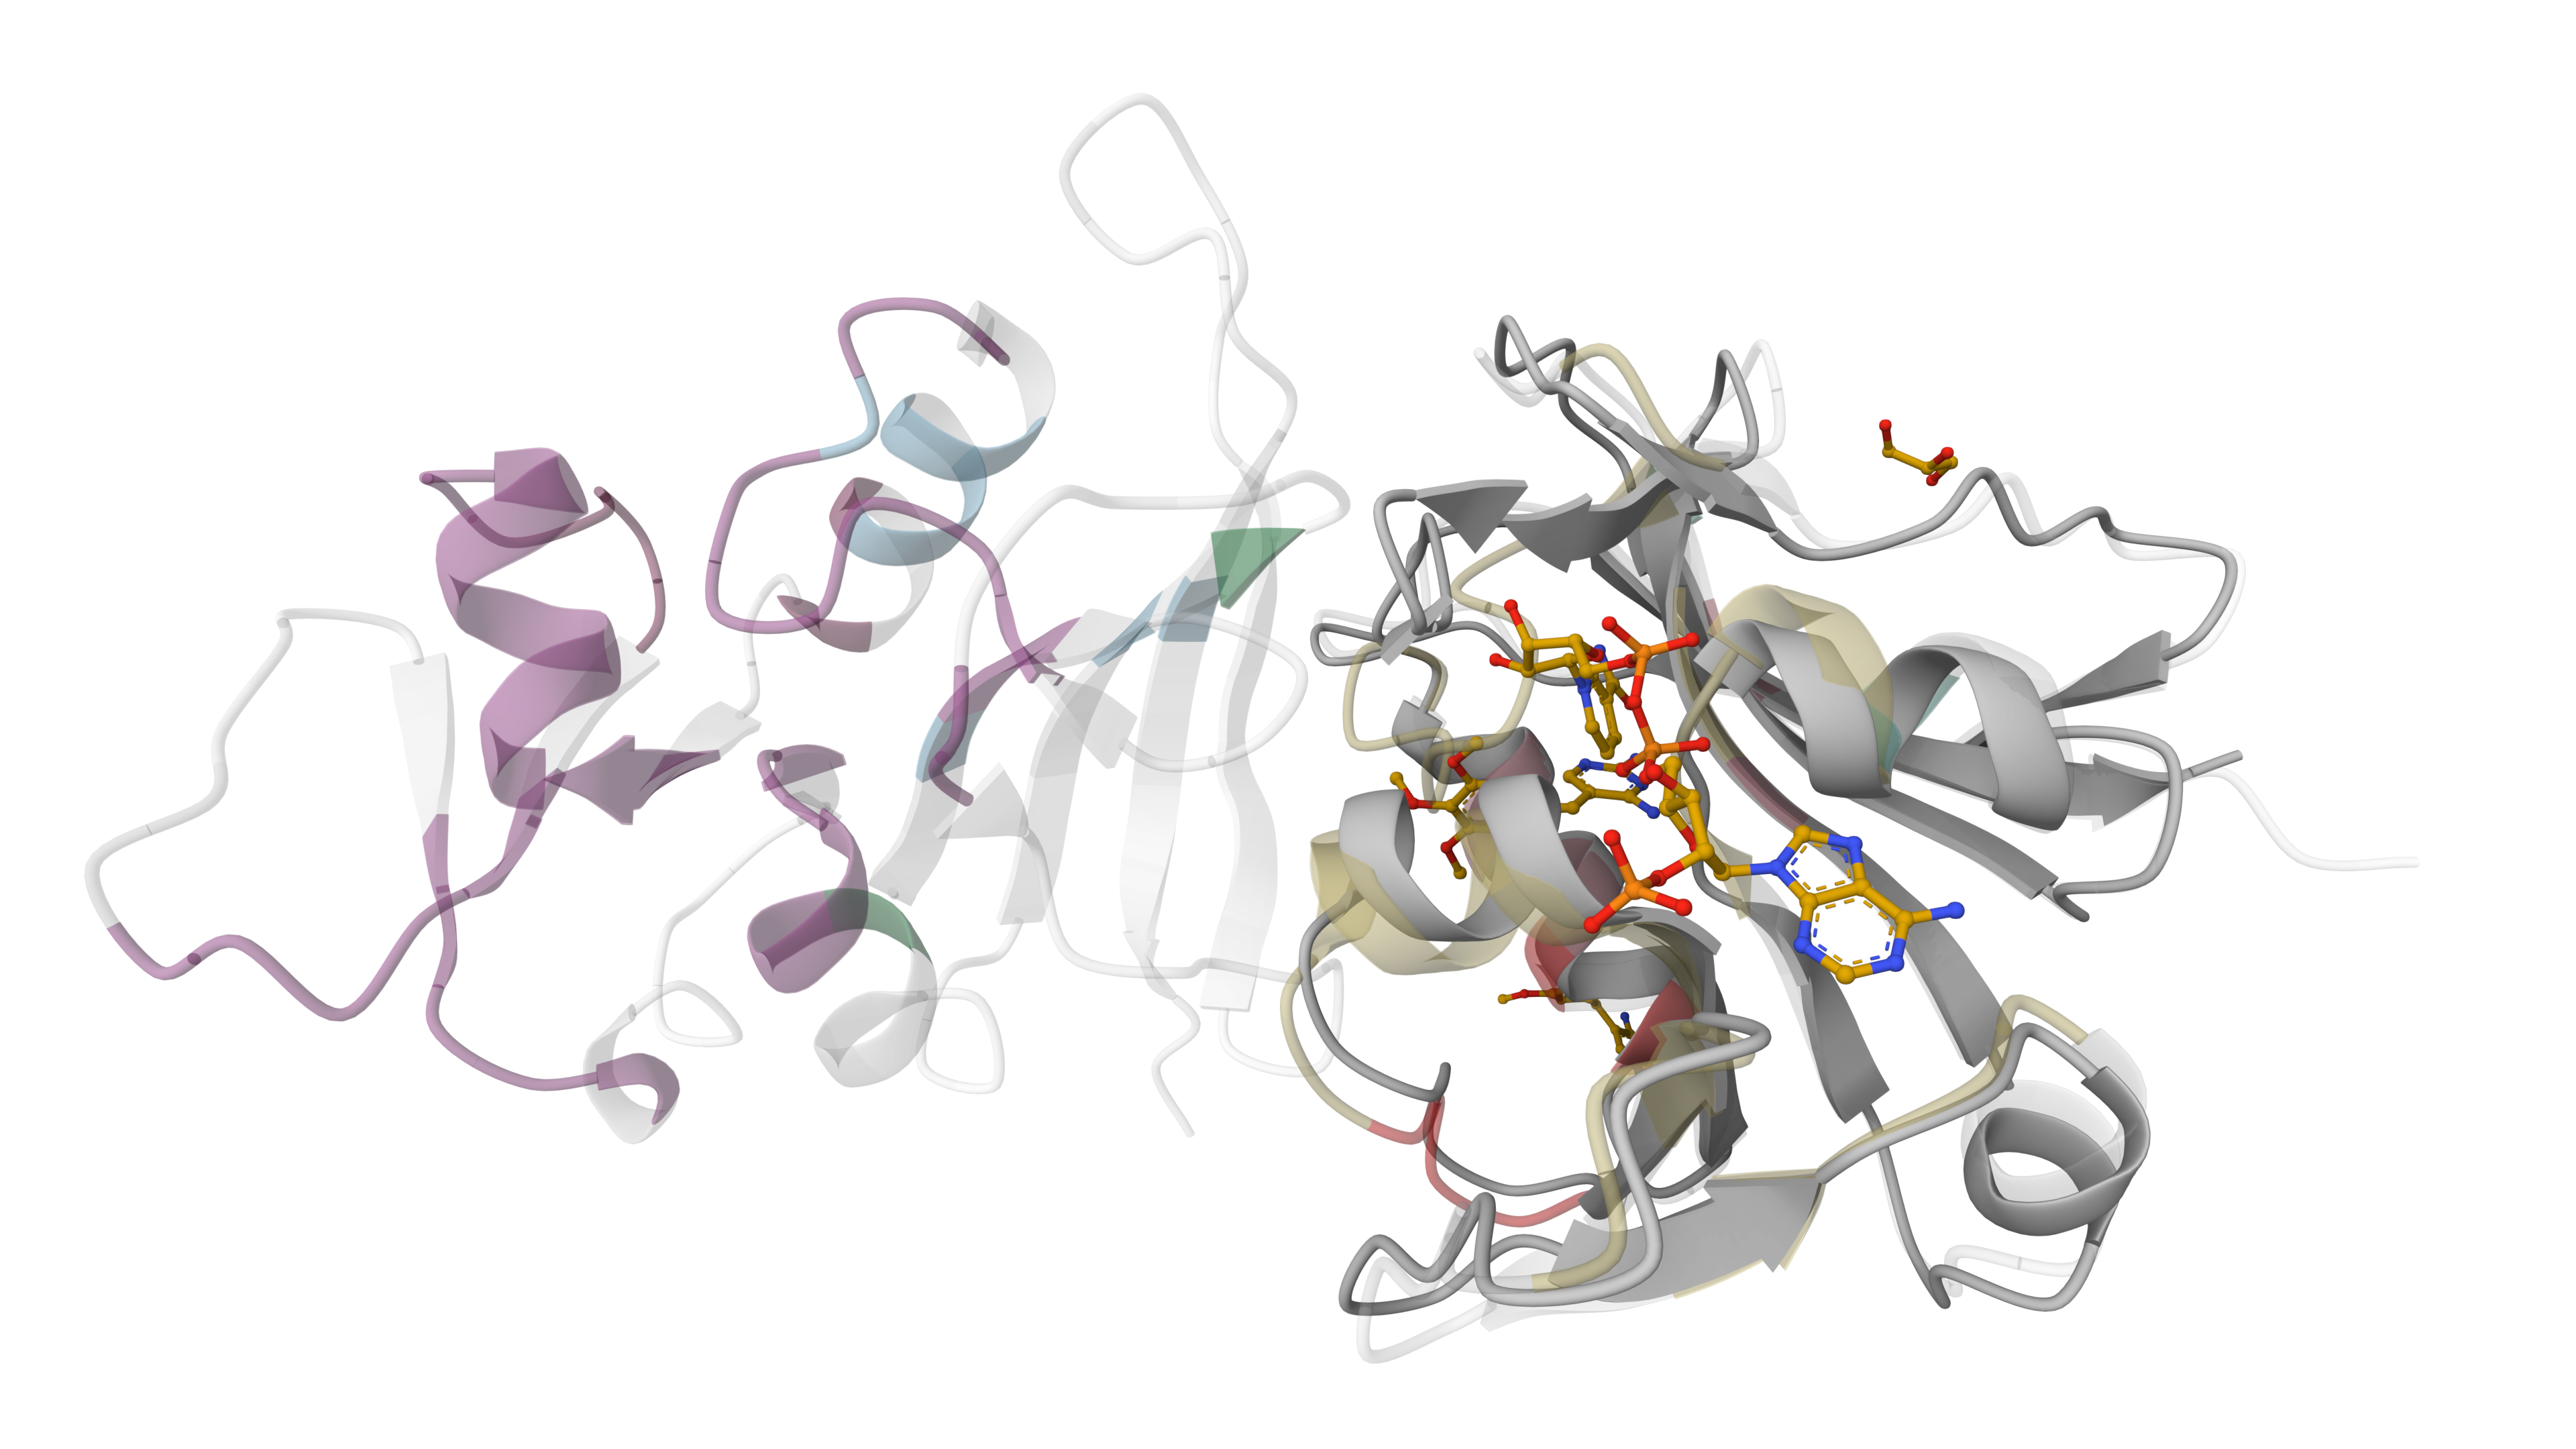
\includegraphics[width=\textwidth]{img/2w9t_2w9s.png}
    \caption{Structural comparison between DHFR apo (2W9T) and holo (2W9S) structures, showing the bound trimethoprim ligand and conformational changes in the Met20 loop region.}
    \label{fig:2w9t_2w9s}
\end{figure}

This comparison between 2W9T (apo) and 2W9S (holo) provides a validation of the cryptic pocket prediction. The application was able to identify a site that is not visible in the apo structure but becomes occupied by a ligand in the holo structure.

\subsection{Further Exploration via Molecular Dynamics}
\label{subsec:md-exploration}

To further investigate the dynamic opening of the predicted pocket, one can perform molecular dynamics (MD) simulations using tools such as GROMACS~\cite{van2005gromacs}, starting from the 2W9T structure. While CryptoShow provides only a brief, illustrative visualization of the conformational change, MD simulations offer a detailed and realistic exploration of the protein's dynamics. During the simulation, the Met20 loop displays conformational flexibility, and the predicted pocket transiently appears. Pocket detection tools such as Fpocket~\cite{le2009fpocket} and TRAPP~\cite{kokh2013trapp} can be used to monitor the pocket's volume and accessibility throughout the simulation.

The results support the idea that the site is not an artifact of ligand binding, but a real conformational feature that may be exploited for inhibitor design and further studies.

\subsection{Use Case Conclusion}
\label{subsec:use-case-conclusion}

This use case demonstrates how the CryptoShow application can be used to predict cryptic binding sites from an apo structure, and how known holo structures, such as 2W9S, can be used to validate the accuracy of those predictions. It highlights the practical application of structural bioinformatics and simulation tools in supporting early-stage drug discovery efforts, demonstrating the real-world utility of the developed application in computational structural biology research.


\chapter*{Conclusion}
\addcontentsline{toc}{chapter}{Conclusion}


%%% Bibliography
%%% Bibliography (literature used as a source)
%%%
%%% We employ biblatex to construct the bibliography. It processes
%%% citations in the text (e.g., the \cite{...} macro) and looks up
%%% relevant entries in the bibliography.bib file.
%%%
%%% See also biblatex settings in thesis.tex.

%%% Generate the bibliography. Beware that if you cited no works,
%%% the empty list will be omitted completely.

% We let bibliography items stick out of the right margin a little
\def\bibfont{\hfuzz=2pt}

\printbibliography[heading=bibintoc]

%%% If case you prefer to write the bibliography manually (without biblatex),
%%% you can use the following. Please follow the ISO 690 standard and
%%% citation conventions of your field of research.

% \begin{thebibliography}{99}
%
% \bibitem{lamport94}
%   {\sc Lamport,} Leslie.
%   \emph{\LaTeX: A Document Preparation System}.
%   2nd edition.
%   Massachusetts: Addison Wesley, 1994.
%   ISBN 0-201-52983-1.
%
% \end{thebibliography}


%%% Figures used in the thesis (consider if this is needed)
\listoffigures

%%% Tables used in the thesis (consider if this is needed)
%%% In mathematical theses, it could be better to move the list of tables to the beginning of the thesis.
\listoftables

%%% List of listings (source code, algorithms, etc.)
\lstlistoflistings

%%% Abbreviations used in the thesis, if any, including their explanation
%%% In mathematical theses, it could be better to move the list of abbreviations to the beginning of the thesis.
\chapwithtoc{List of Abbreviations}

\xxx{TODO}

%%% Doctoral theses must contain a list of author's publications
\ifx\ThesisType\TypePhD
\chapwithtoc{List of Publications}
\fi

%%% Attachments to the thesis, if any. Each attachment must be referred to
%%% at least once from the text of the thesis. Attachments are numbered.
%%%
%%% The printed version should preferably contain attachments, which can be
%%% read (additional tables and charts, supplementary text, examples of
%%% program output, etc.). The electronic version is more suited for attachments
%%% which will likely be used in an electronic form rather than read (program
%%% source code, data files, interactive charts, etc.). Electronic attachments
%%% should be uploaded to SIS. Allowed file formats are specified in provision
%%% of the rector no. 72/2017. Exceptions can be approved by faculty's coordinator.
\appendix
\chapter{Attachments}

\section{Source Codes}
\label{sec:source-codes}

\xxx{TODO: source codes}

\section{Web Application}
\label{sec:web-application}

The CryptoShow web application is available at \url{https://cryptoshow.cz/}.

\section{API Endpoints}
\label{sec:api-endpoints}

The following table summarizes the API endpoints exposed by the FastAPI server.

\begin{itemize}
    \item \textbf{GET /} - Root endpoint, returns a hello message for debugging.
    \item \textbf{GET /openapi} - Returns the generated OpenAPI schema for the API.
    \item \textbf{GET /gpu-status} - Checks if CUDA is available; returns a task ID for the CUDA Celery test task.
    \item \textbf{GET /health} - Returns the health status of the server (\lstinline|status: healthy|).
    \item \textbf{POST /calculate} - Calculates the prediction for a given PDB/AF ID.
    \item \textbf{POST /calculate-custom} - Calculates the prediction for an uploaded PDB/mmCIF file.
    \item \textbf{GET /task-status/\{task\_id\}} - Checks the status of a Celery task. Returns status and result if available.
    \item \textbf{GET /file/\{task\_hash\}/\{filename\}} - Downloads a file (e.g., results) for a given task.
    \item \textbf{GET /animate/\{task\_hash\}/\{aligned\_structure\_filename\}/\{target\_chains\}} - Creates an animated trajectory file for selected chains and a given structure file.
    \item \textbf{WS /ws/task-status/\{task\_id\}} - WebSocket endpoint for real-time Celery task status updates.
    \item \textbf{POST /proxy/ahoj/job} - Proxies a POST request to \lstinline|apoholo.cz| for job submission.
    \item \textbf{GET /proxy/ahoj/\{task\_hash\}/\{path\}} - Proxies a GET request to \lstinline|apoholo.cz| for file retrieval.
\end{itemize}


\end{document}
